% This presentation uses Aalborg Beamer Theme http://kom.aau.dk/~jkn/latex/latex.php#beamer_aausidebar
\documentclass[12pt, aspectratio=1610]{beamer}
\usetheme[
%%% options passed to the outer theme
hidetitle,           % hide the (short) title in the sidebar
    hideauthor,          % hide the (short) author in the sidebar
%    hideinstitute,       % hide the (short) institute in the bottom of the sidebar
%    shownavsym,          % show the navigation symbols
%    width=2cm,           % width of the sidebar (default is 2 cm)
    hideothersubsections,% hide all subsections but the subsections in the current section
%    hideallsubsections,  % hide all subsections
%    left                % right of left position of sidebar (default is right)
  ]{Aalborg}
  
% If you want to change the colors of the various elements in the theme, edit and uncomment the following lines
% Change the bar and sidebar colors:
\definecolor{MyBlue}{RGB}{0,53,107}
\definecolor{MyLightBlue}{RGB}{0,53,107}
\definecolor{MyGray}{RGB}{102,102,102}
\setbeamercolor{Aalborg}{fg=MyLightBlue!50, bg=MyBlue}
%\setbeamercolor{sidebar}{bg=red!20}
% Change the color of the structural elements:
\setbeamercolor{structure}{fg=MyBlue}
% Change the frame title text color:
\setbeamercolor{frametitle}{fg=MyBlue}
\setbeamercolor{titlepagecolorbox}{fg=white,bg=MyBlue}
% Change the normal text color background:
%\setbeamercolor{normal text}{fg=gray!50}
% ... and you can of course change a lot more - see the beamer user manual.

\usepackage[utf8]{inputenc}
\usepackage[english, ukrainian]{babel}
\usepackage[T1, T2A]{fontenc}
% Or whatever. Note that the encoding and the font should match. If T1
% does not look nice, try deleting the line with the fontenc.
\usepackage{droid}


% colored hyperlinks
\newcommand{\chref}[2]{%
  \href{#1}{{\usebeamercolor[bg]{Aalborg}#2}}%
}

% footnotes without markers
\newcommand\blfootnote[1]{%
	\begingroup
	\renewcommand\thefootnote{}\footnote{#1}%
	\addtocounter{footnote}{-1}%
	\endgroup
}

\title[Структура природно-заповідного фонду України]% optional, use only with long paper titles
{Структура природно-заповідного фонду України}

\subtitle{попередні результати аналізу відкритих даних\\
	      Міністерства екології та природних ресурсів}  % could also be a conference name

\date[23 лютого 2017 р.]{\vspace{-1.5 mm} 23 лютого 2017 р.\\
	                    {\href{http://gis-forum.org.ua/}
	                    {\vspace{-1.5 mm}\scriptsize ГІС-форум: Освіта Наука Виробництво}\\
                        {\scriptsize м. Харків, Україна}}}
                                        
\author[Дар'я Свідзінська] % optional, use only with lots of authors
{
  Дар'я Свідзінська\\
  \href{mailto:d.svidzinska@gmail.com}{{\tt d.svidzinska@gmail.com}}
}

\institute[
%  {\includegraphics[scale=0.2]{aau_segl}}\\ %insert a company, department or university logo
  % Кафедра фізичної географії та геоекології\\
  % Лабораторія GeoForAll\\
  % Київський національний університет імені Тараса Шевченка
] % optional - is placed in the bottom of the sidebar on every slide
{% is placed on the bottom of the title page
  Кафедра фізичної географії та геоекології\\
  \href{http://lab.osgeo.org.ua/}{Лабораторія GeoForAll}\\
  Київський національний університет імені Тараса Шевченка
  
  %there must be an empty line above this line - otherwise some unwanted space is added between the university and the country (I do not know why;( )
}


% specify the logo in the top right/left of the slide
%\pgfdeclareimage[height=1cm]{mainlogo}{AAUgraphics/aau_logo_new} % placed in the upper left/right corner
%\logo{\pgfuseimage{mainlogo}}

% specify a logo on the titlepage (you can specify additional logos an include them in 
% institute command below
% \pgfdeclareimage[height=1.5cm]{titlepagelogo}{AAUgraphics/tsnuk_logo} % placed on the title page
% \pgfdeclareimage[height=1.5cm]{titlepagelogo2}{AAUgraphics/lab_logo} % placed on the title page
% \titlegraphic{% is placed on the bottom of the title page
	%\pgfuseimage{titlepagelogo}
	%\hspace{0.5cm}\pgfuseimage{titlepagelogo2}
%}

\begin{document}
% the titlepage
{%\aauwavesbg
\begin{frame}[plain,noframenumbering] % the plain option removes the sidebar and header from the title page
  \titlepage
\end{frame}}
%%%%%%%%%%%%%%%%

% TOC
%\begin{frame}[allowframebreaks]{Зміст}{}
%\setcounter{tocdepth}{2}
%\tableofcontents
%\end{frame}
%%%%%%%%%%%%%%%%
\newcommand{\quoteTitle}[3]{%
	\href{#3}%
	{\emph{#1}\\%
		\hfill%
		{\footnotesize#2}%
		\smallskip}%
}
\newcommand{\quoteText}[3]{\quoteTitle{#1}{#2}{#3}}

\section{Передумови}
% motivation
\begin{frame}{Передумови}{}
\quoteTitle{розширення площі природно-заповідного фонду до \alert{15\%} загальної території країни у \alert{2020} році}%
           {Про Основні засади (стратегію) державної екологічної політики України на період до 2020 року, 2010}%
           {http://zakon2.rada.gov.ua/laws/show/2818-17}
\end{frame}
%%%%%%%%%%%%%%%%

%\subsection{Організація системи обліку}
% the license
%\begin{frame}{Передумови}{Організація системи обліку}
 %\begin{block}{Державний кадастр територій та об'єктів ПЗФ}
     	%\quoteTitle{формами кадастрової документації є \alert{картки первинного обліку}}%
     	%{Про природно-заповідний фонд України, 1992}%
     	%{http://zakon5.rada.gov.ua/laws/show/2456-12}  	
 %\end{block}
 %\begin{block}{Інші типи документації}
 	%\begin{itemize}
 		%\item рішення про створення
 		%\item охоронне зобов'язання
 		%\item положення
 	%\end{itemize}
 %\end{block}
%\end{frame}
%%%%%%%%%%%%%%%%

\subsection{Існуюча система обліку}
\begin{frame}{Передумови}{Існуюча система обліку}
		\begin{itemize}
			\item розкиданість інформації
			\item неповнота документації
			\item недостовірність
			\item застарілість
			\item відсутність геоданих
			\item відсутність відкритого доступу
		\end{itemize}
\end{frame}
%%%%%%%%%%%%%%%%

\subsection{Джерело інформації}
\begin{frame}{Передумови}{Джерело інформації}
 \begin{block}{\href{http://data.gov.ua/passport/9e011264-c16d-42ab-95f1-b06f7311103e}{Перелік територій та об'єктів природно-заповідного фонду загальнодержавного та місцевого значення в розрізі адміністративно-територіальних одиниць}}
	\begin{itemize}
		\item розпорядник інформації -- Міністерство екології та природних ресурсів України
		\item відкритий доступ через \href{http://data.gov.ua/passport/9e011264-c16d-42ab-95f1-b06f7311103e}{Єдиний державний веб-портал відкритих даних}
		\item запланована частота оновлення -- 1 раз на рік
	\end{itemize}
 \end{block}
\end{frame}
%%%%%%%%%%%%%%%%

\section{Завдання роботи}
% основні завдання роботи
\begin{frame}{Завдання роботи}
   \begin{enumerate}
    \item оцінити якість даних
    \item впорядкувати дані\footnote{за потреби}
    \item проаналізувати структуру природно-заповідного фонду
   \end{enumerate}
  \begin{block}{Для чого}
  	\begin{itemize}
  		\item потреба в актуальній статистиці
  		\begin{itemize}
  			\item для викладання
  			\item для проектів
  		\end{itemize}
  	    \item just curious {\tt :)}
  	\end{itemize}
  \end{block}
\end{frame}
%%%%%%%%%%%%%%%%

\section{Оцінка якості даних}
\subsection{Доступність}
\begin{frame}{Оцінка якості даних}{Доступність}
\subsubsection{Умови використання}	
	\begin{block}{Умови використання}
	\quoteTitle{Будь-яка особа може вільно копіювати, публікувати, поширювати, використовувати, у тому числі в комерційних цілях, у поєднанні з іншою інформацією або шляхом включення до складу власного продукту, публічну інформацію у формі відкритих даних з обов'язковим посиланням на джерело отримання такої інформації.}%
	{Єдиний державний веб-портал відкритих даних}%
	{http://data.gov.ua/}  
	\end{block}
\end{frame}
%%%%%%%%%%%%%%%%

\begin{frame}{Оцінка якості даних}{Доступність}
	\subsubsection{Завантаження}
	\begin{block}{Завантаження}
		\begin{itemize}
			\item доступне <<традиційне>> завантаження
			\item за API -- непридатні для обробки {\tt xml}-файли
			\item найменування файлів нестандартизовані
		\end{itemize} 
	\end{block}
\end{frame}
%%%%%%%%%%%%%%%%

\subsection{Актуальність}
\begin{frame}{Оцінка якості даних}{Актуальність}
	\begin{itemize}
			\item перше оприлюднення -- 15.02.2016
			\item останні зміни -- 12.04.2016
			\item інформація станом на \alert{01.01.2015}
			\item запланована частота оновлення -- 1 раз на рік
	\end{itemize} 
\end{frame}
%%%%%%%%%%%%%%%%

\subsection{Чистота}
\begin{frame}{Оцінка якості даних}{Чистота}
	\subsubsection{Поняття чистих даних}	
	\begin{block}{Чисті дані\footnote{оскільки \alert{жодна} з цих умов не виконана, \alert{90\%} робочого часу пішло на очищення та структурування даних}}
	\begin{itemize}
		\item не містять помилок та одруківок
		\item в межах одного типу чи класу мають уніфікований формат
		\item назви всюди пишуться однаково
		\item не містять об'єднаних комірок
	\end{itemize}
\quoteTitle{}%
{Відкритий посібник з відкритих даних, 2016}%
{http://socialdata.org.ua/manual3/}
\end{block}
\end{frame}
%%%%%%%%%%%%%%%%

\subsection{Повнота}
\begin{frame}{Оцінка якості даних}{Повнота}
	\begin{center}
	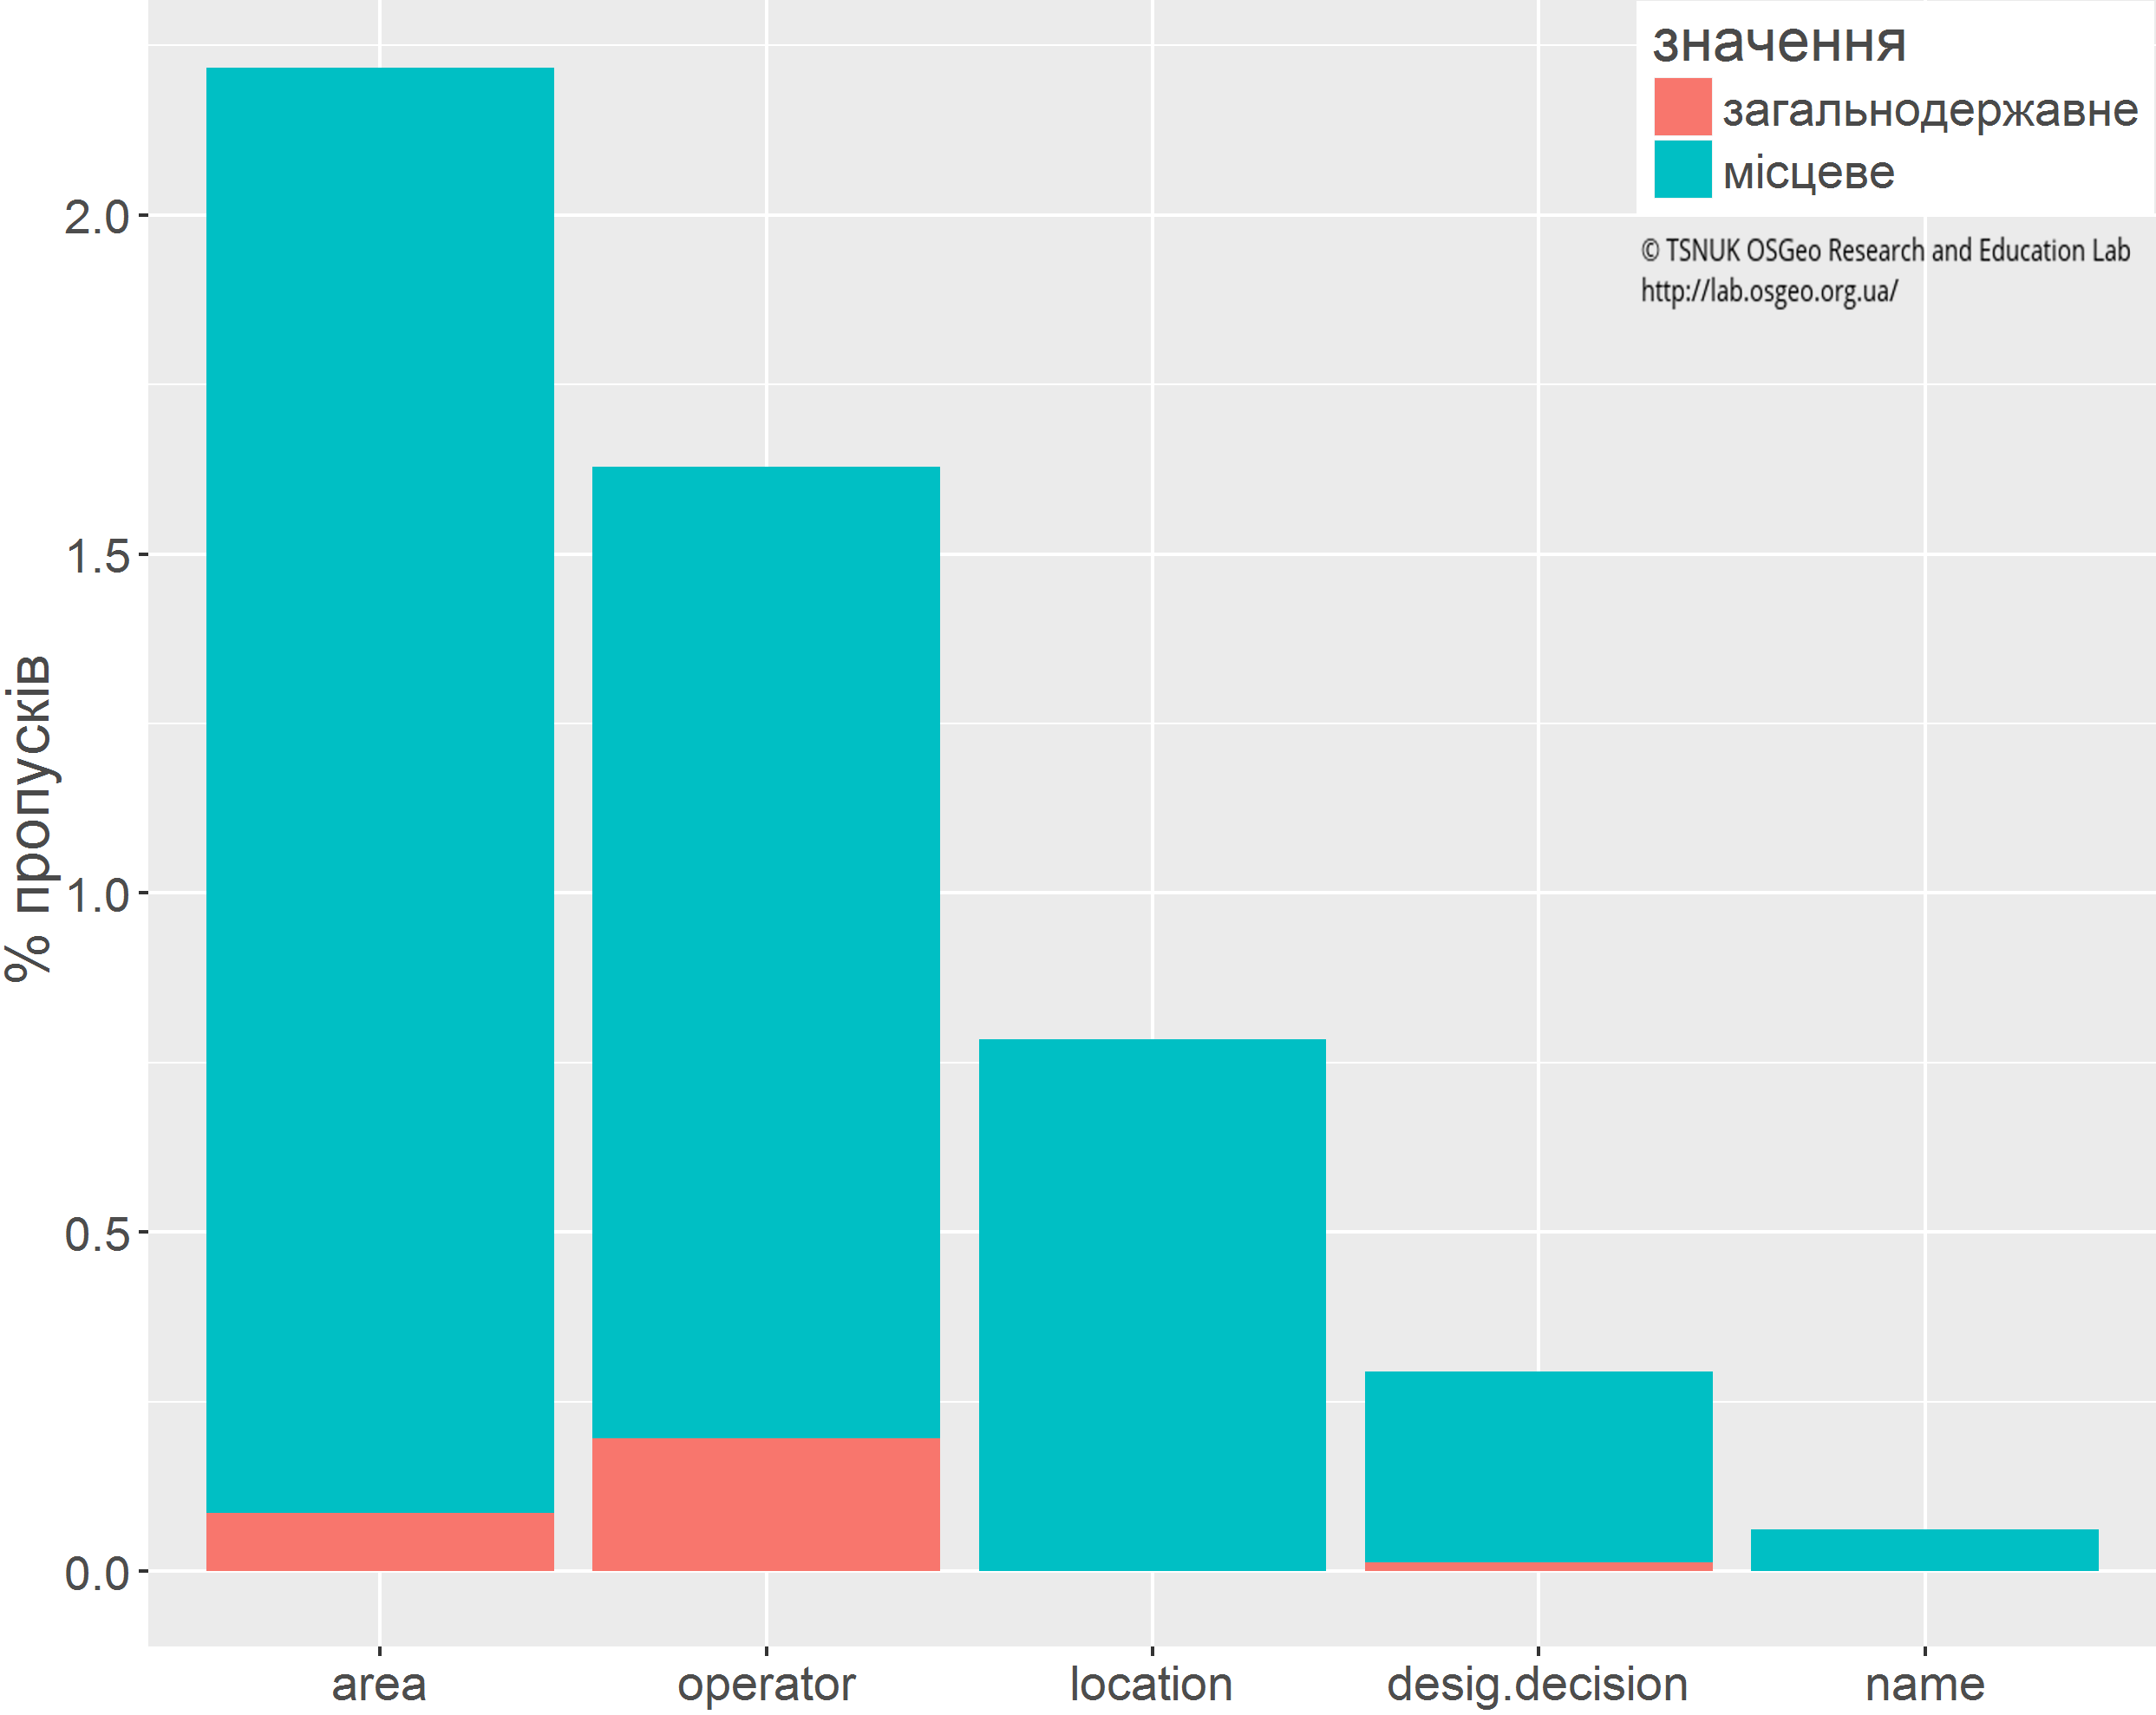
\includegraphics[height=0.72\textheight]{./figures/simple_completeness_graph.png}
	\blfootnote{\tiny{поля \texttt{category} та \texttt{type} проходили додаткову ручну перевірку}}
	\end{center}
\end{frame}
%%%%%%%%%%%%%%%%

\section{Очищення та структурування даних}
\subsection{Що було зроблено}
\begin{frame}{Очищення та структурування даних}{Що було зроблено}
		\begin{enumerate}
			\item скрипт для автоматизованого завантаження даних\blfootnote{\tiny{всі скрипти, проміжні та результуючі дані доступні з репозиторію  \chref{https://github.com/darsvid/menr_pa_data/}{\texttt{https://github.com/darsvid/menr\_pa\_data/}}}}
			\begin{itemize}
				\item стандартизація найменування файлів
				\item часова мітка \texttt{last-modified}
			\end{itemize}
			\item ручне передоброблення
			\begin{itemize}
				\item заповнення пропусків в полях \texttt{type} та \texttt{category}
				\item філії степових заповідників
				\item \href{https://github.com/darsvid/menr_pa_data/blob/master/messy_data_01/readme.md}{інше}
			\end{itemize}
			\item автоматизоване оброблення
			\begin{itemize}
				\item поле \texttt{importance}
				\item видалення підсумовувальних рядків
				\item видалення надлишкових символів з полів \texttt{name, desig.decision, operator, location}
				\item стандартизація полів \texttt{category} та \texttt{type}
			\end{itemize}
		\end{enumerate}
\end{frame}
%%%%%%%%%%%%%%%%

\subsection{Що планується зробити}
\begin{frame}{Очищення та структурування даних}{Що планується зробити}
	\begin{itemize}
		\item аналіз дат \texttt{desig.decision}
		\item аналіз установ та організацій \texttt{operator}
		\item підготовка рекомендацій для розпорядника даних
	\end{itemize}
\end{frame}
%%%%%%%%%%%%%%%%

\section{Структура природно-заповідного фонду}

\subsection{Скільки всього об'єктів?}
\begin{frame}{Структура природно-заповідного фонду}{Скільки всього об'єктів?}
	\begin{itemize}
		\item всього 8 164 об'єкти\footnote{філії та території в межах декількох областей представлені, як окремі об'єкти}
		\item загальна площа 40 149.44 км\textsuperscript{2}
		\item 6.65\% від загальної площі країни\footnote{завищене значення без урахування дублювання вкладених площ та акваторій}
	\end{itemize}
\end{frame}
%%%%%%%%%%%%%%%%

\subsection{Як розподіляються об'єкти?}
\begin{frame}{Структура природно-заповідного фонду}{Як розподіляються об'єкти?}
	\begin{columns}[c]
		
		\column{.48\textwidth}
		
		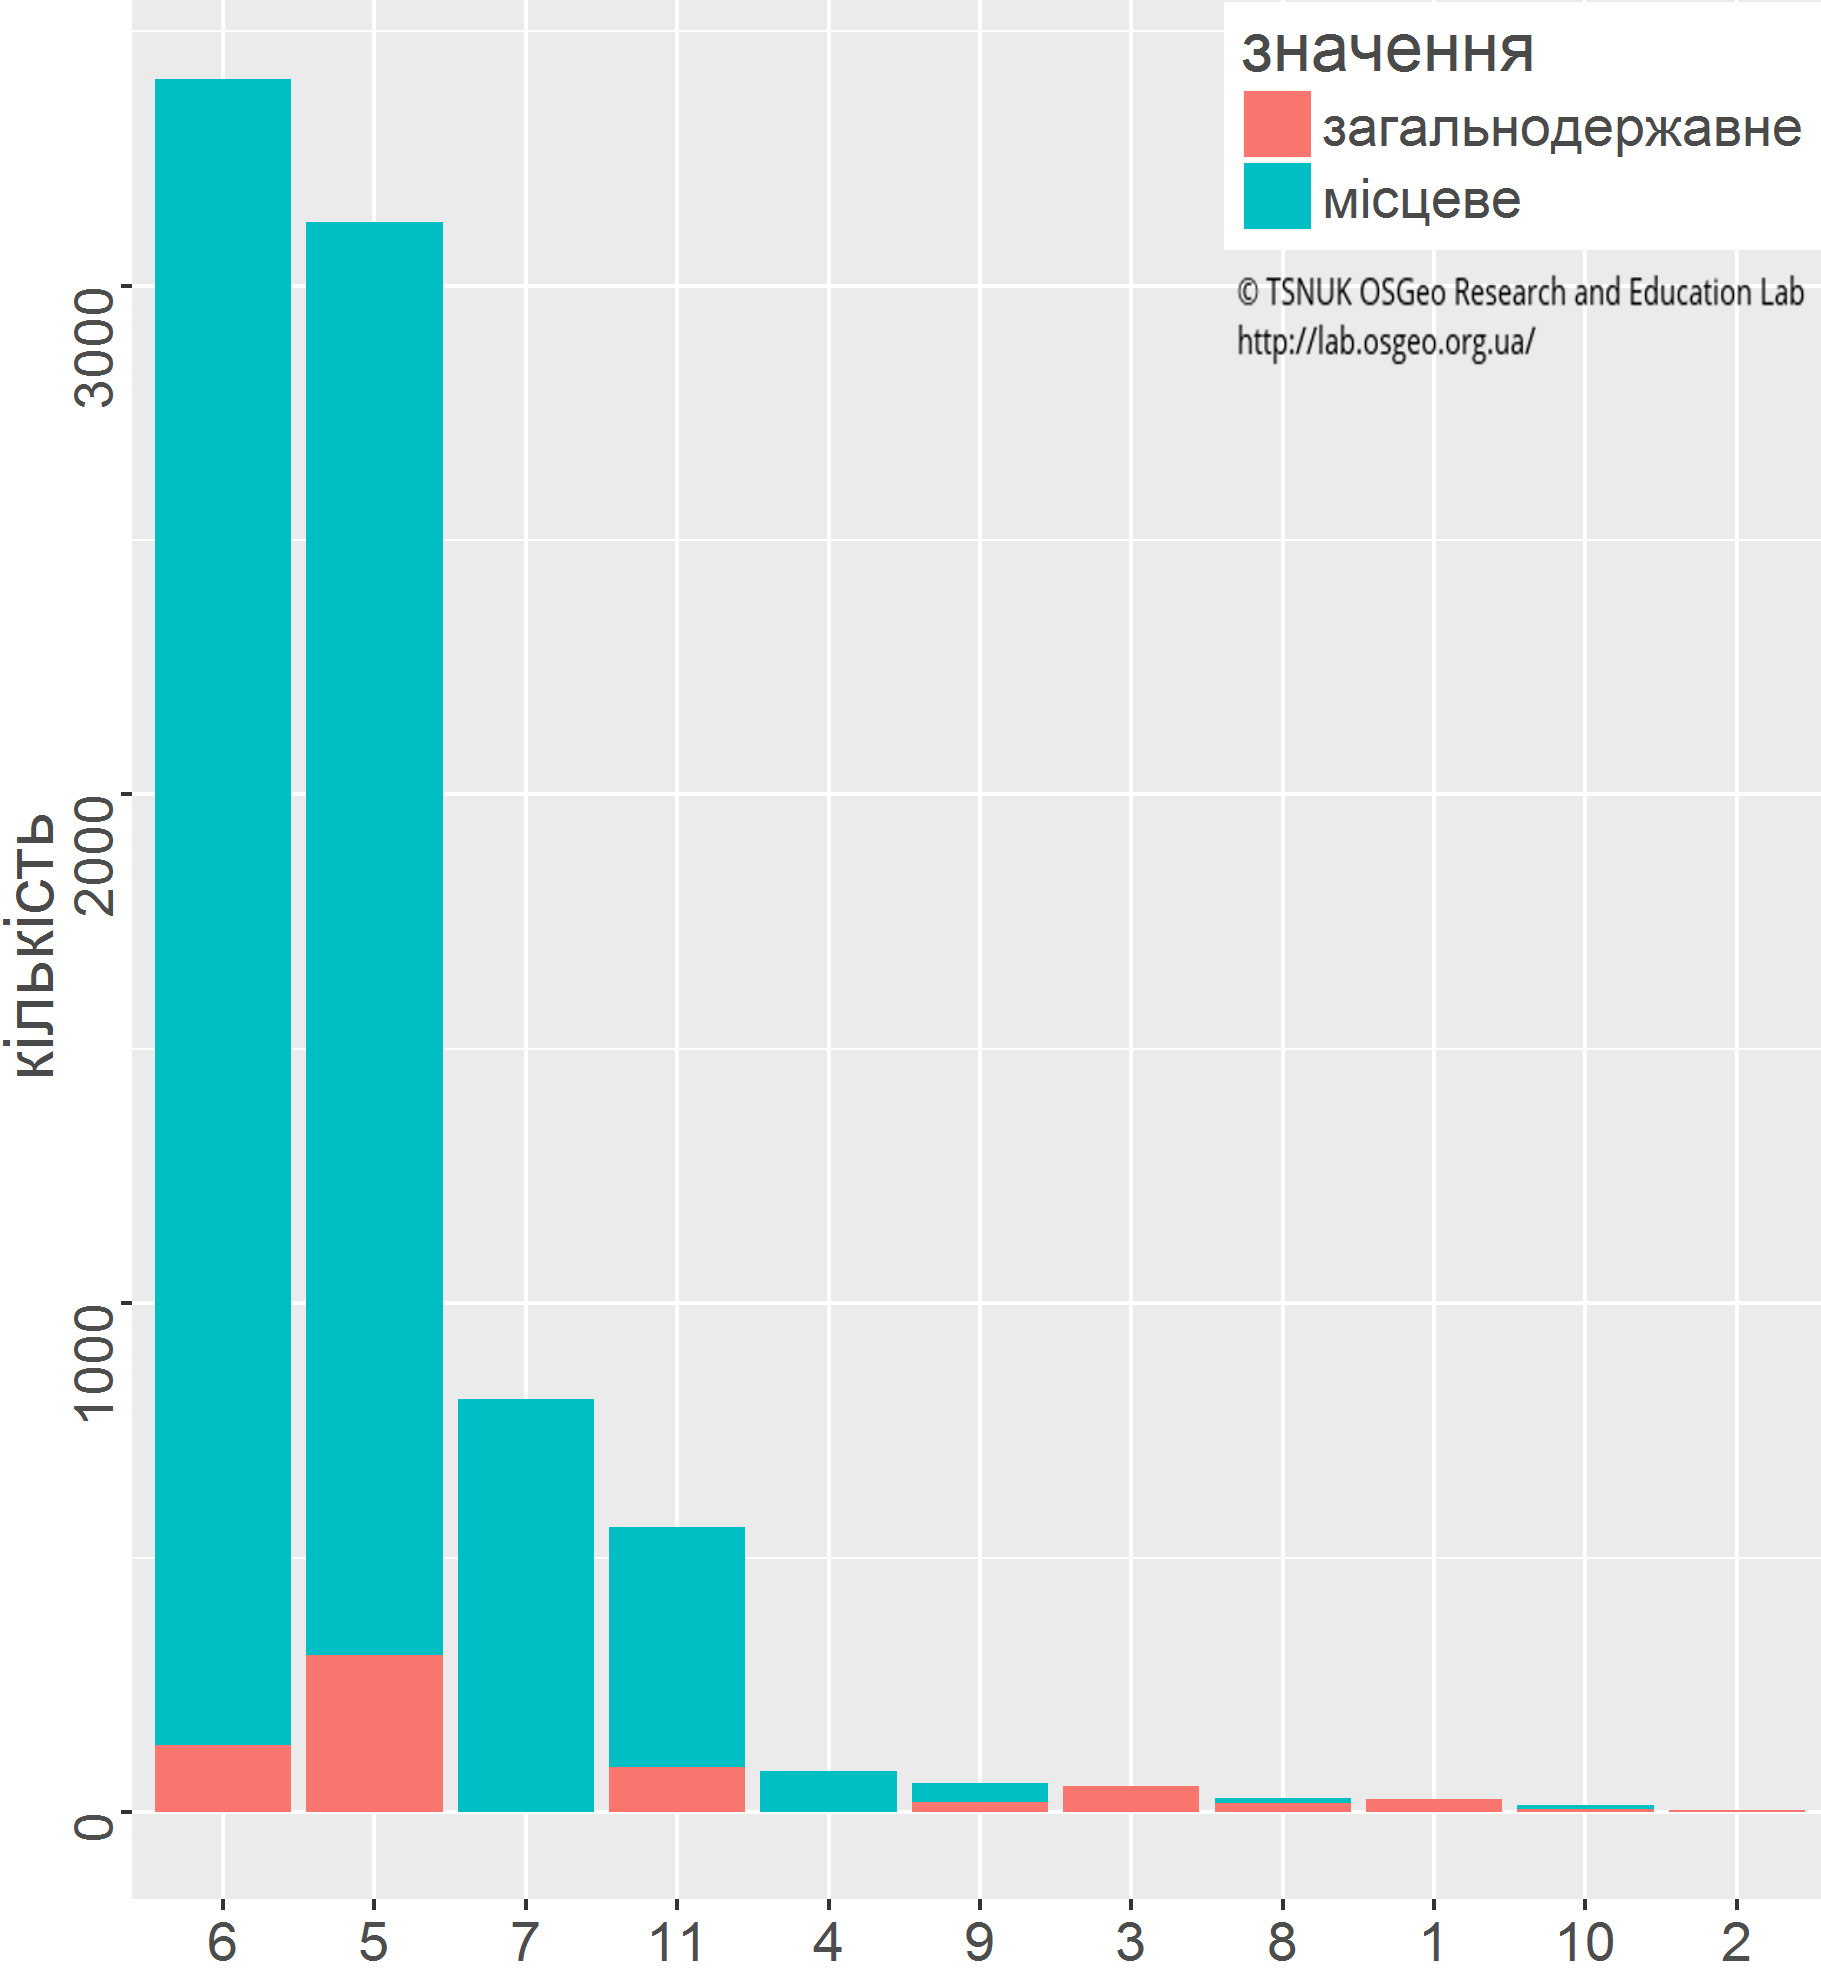
\includegraphics[width=\textwidth]{./figures/quantity.png}%
		
		\column{.48\textwidth}
		
		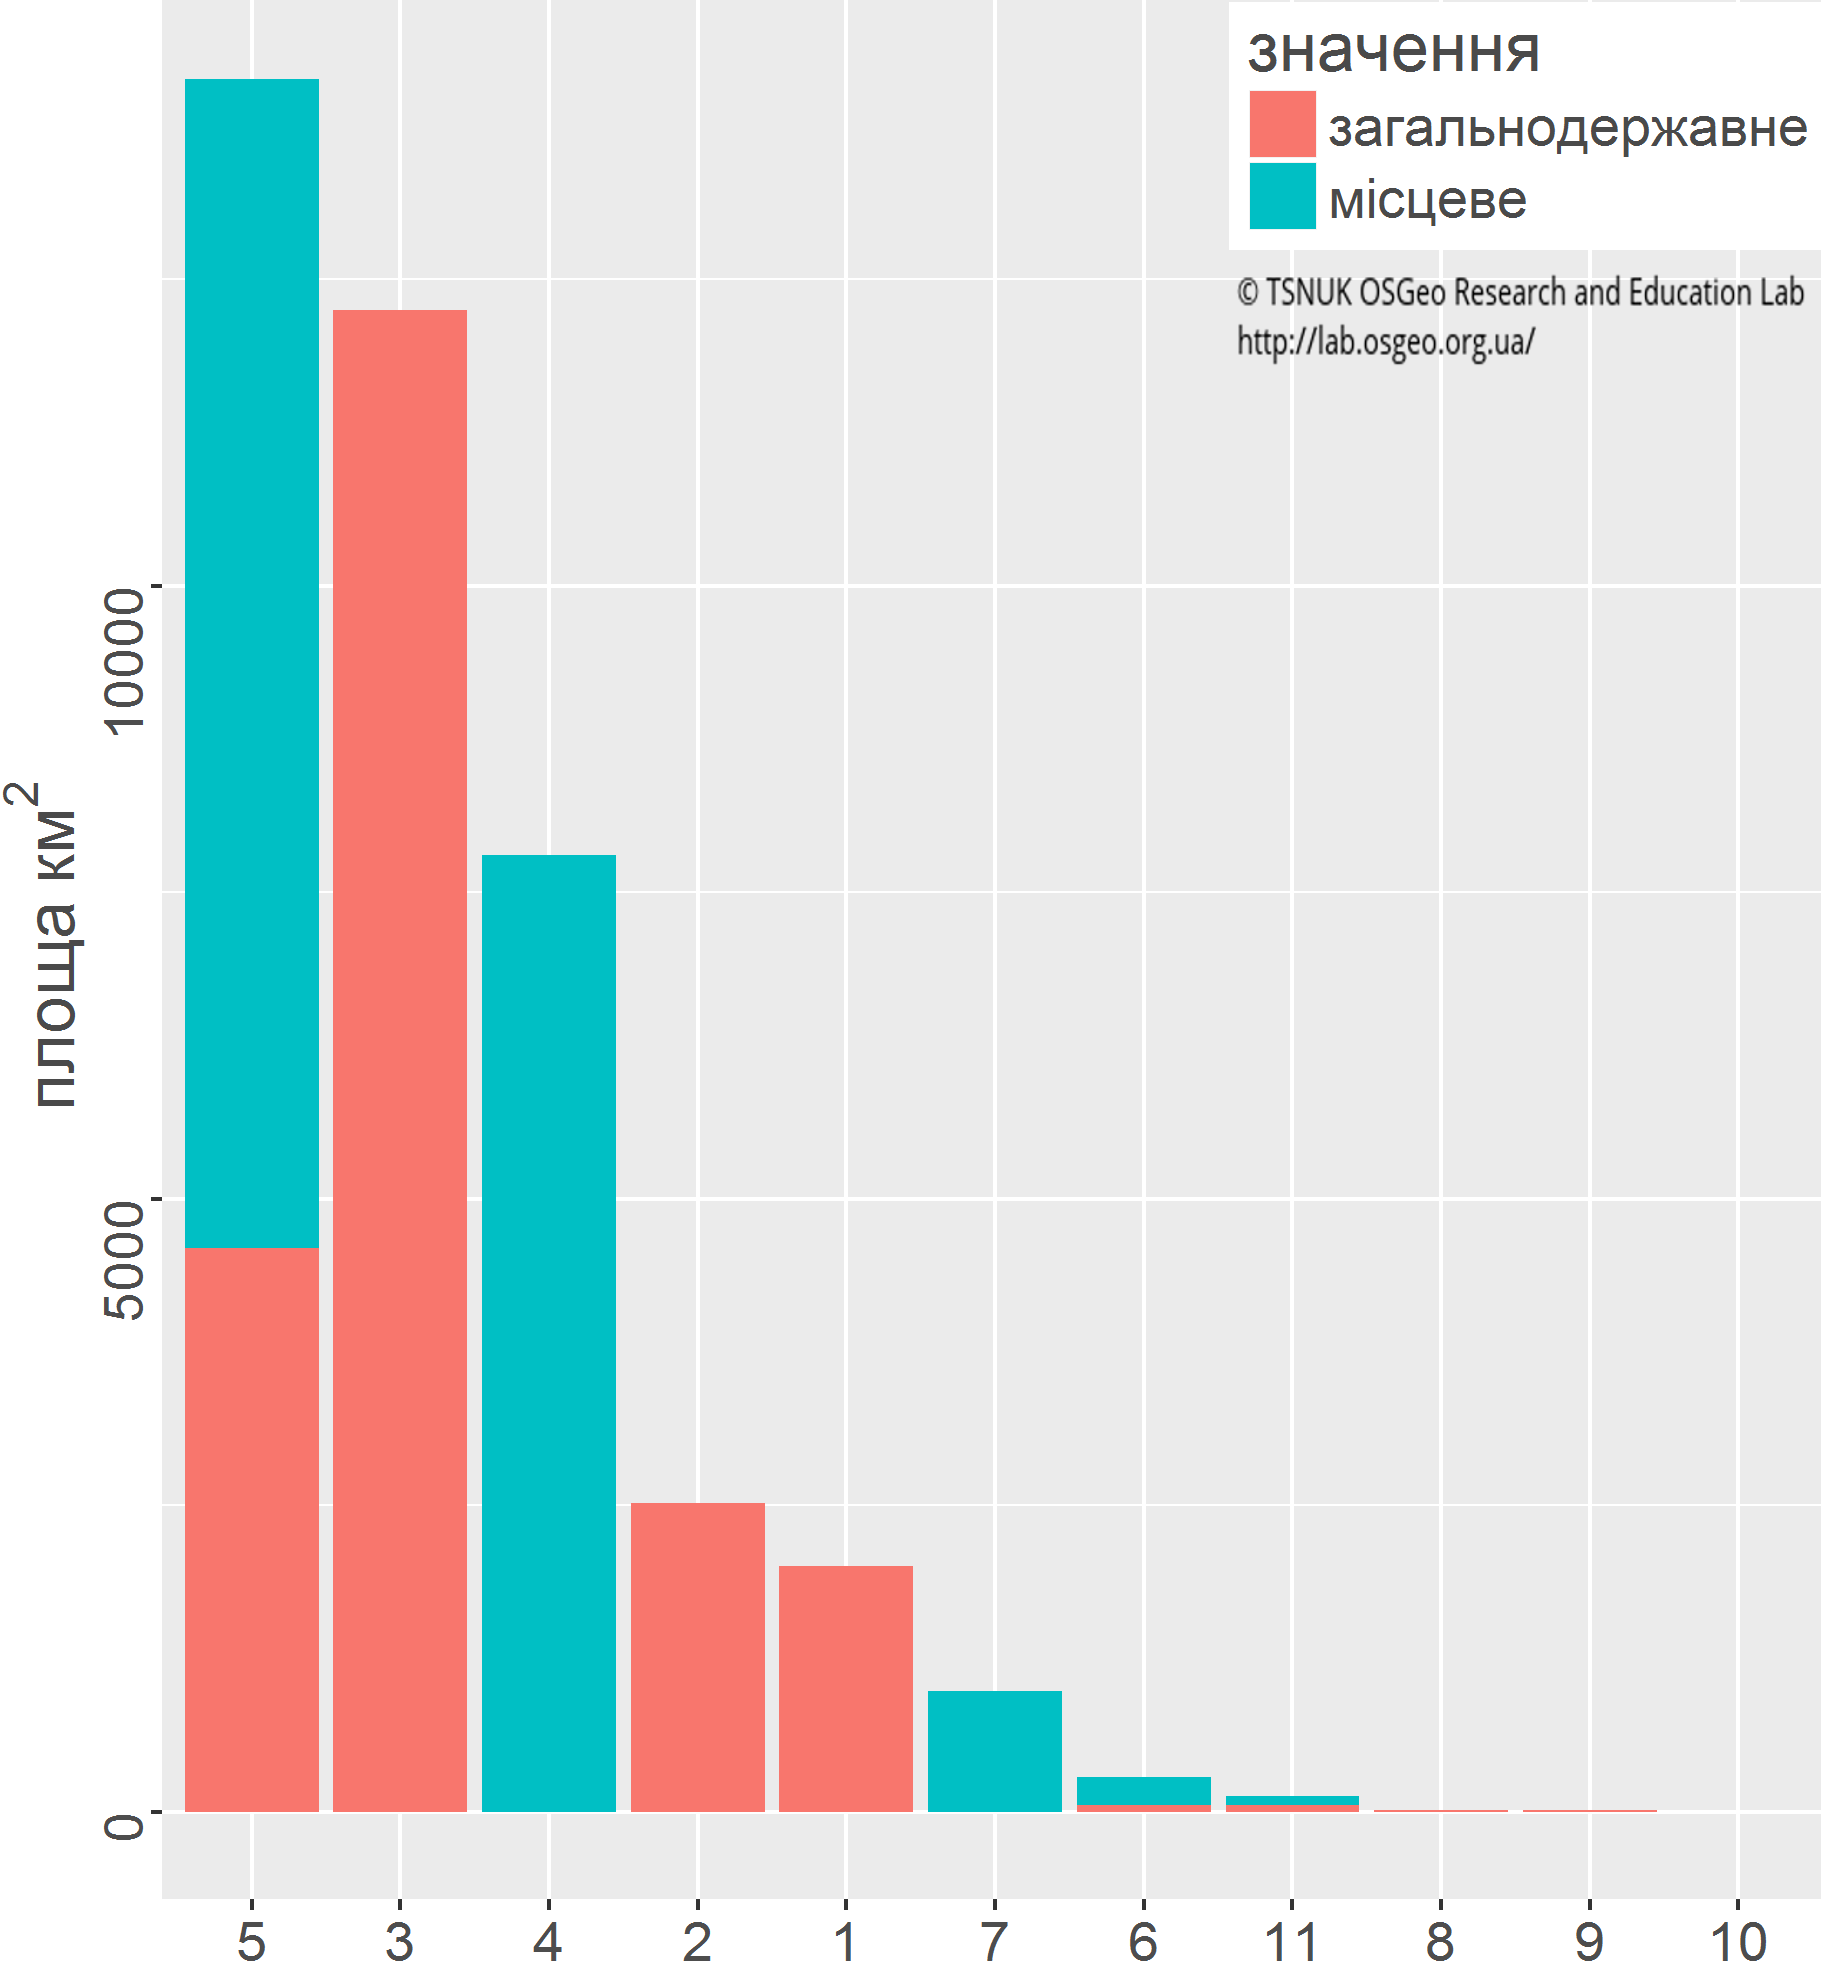
\includegraphics[width=\textwidth]{./figures/area.png}
			
\end{columns}
\blfootnote{\tiny{1 -- природний заповідник, 2 -- біосферний заповідник, 3 -- національний природний парк, 4 -- регіональний ландшафтний парк, 5 -- заказник, 6 -- пам’ятка природи, 7 -- заповідне урочище, 8 -- ботанічний сад, 9 -- дендрологічний парк, 10 -- зоологічний парк, 11 -- парк-пам’ятка садово-паркового мистецтва}}	
\end{frame}

\subsection{Як розподіляються об'єкти за значенням?}
\begin{frame}{Структура природно-заповідного фонду}{Як розподіляються об'єкти за значенням?}
	\begin{columns}[c]
		
		\column{.5\textwidth}
		
		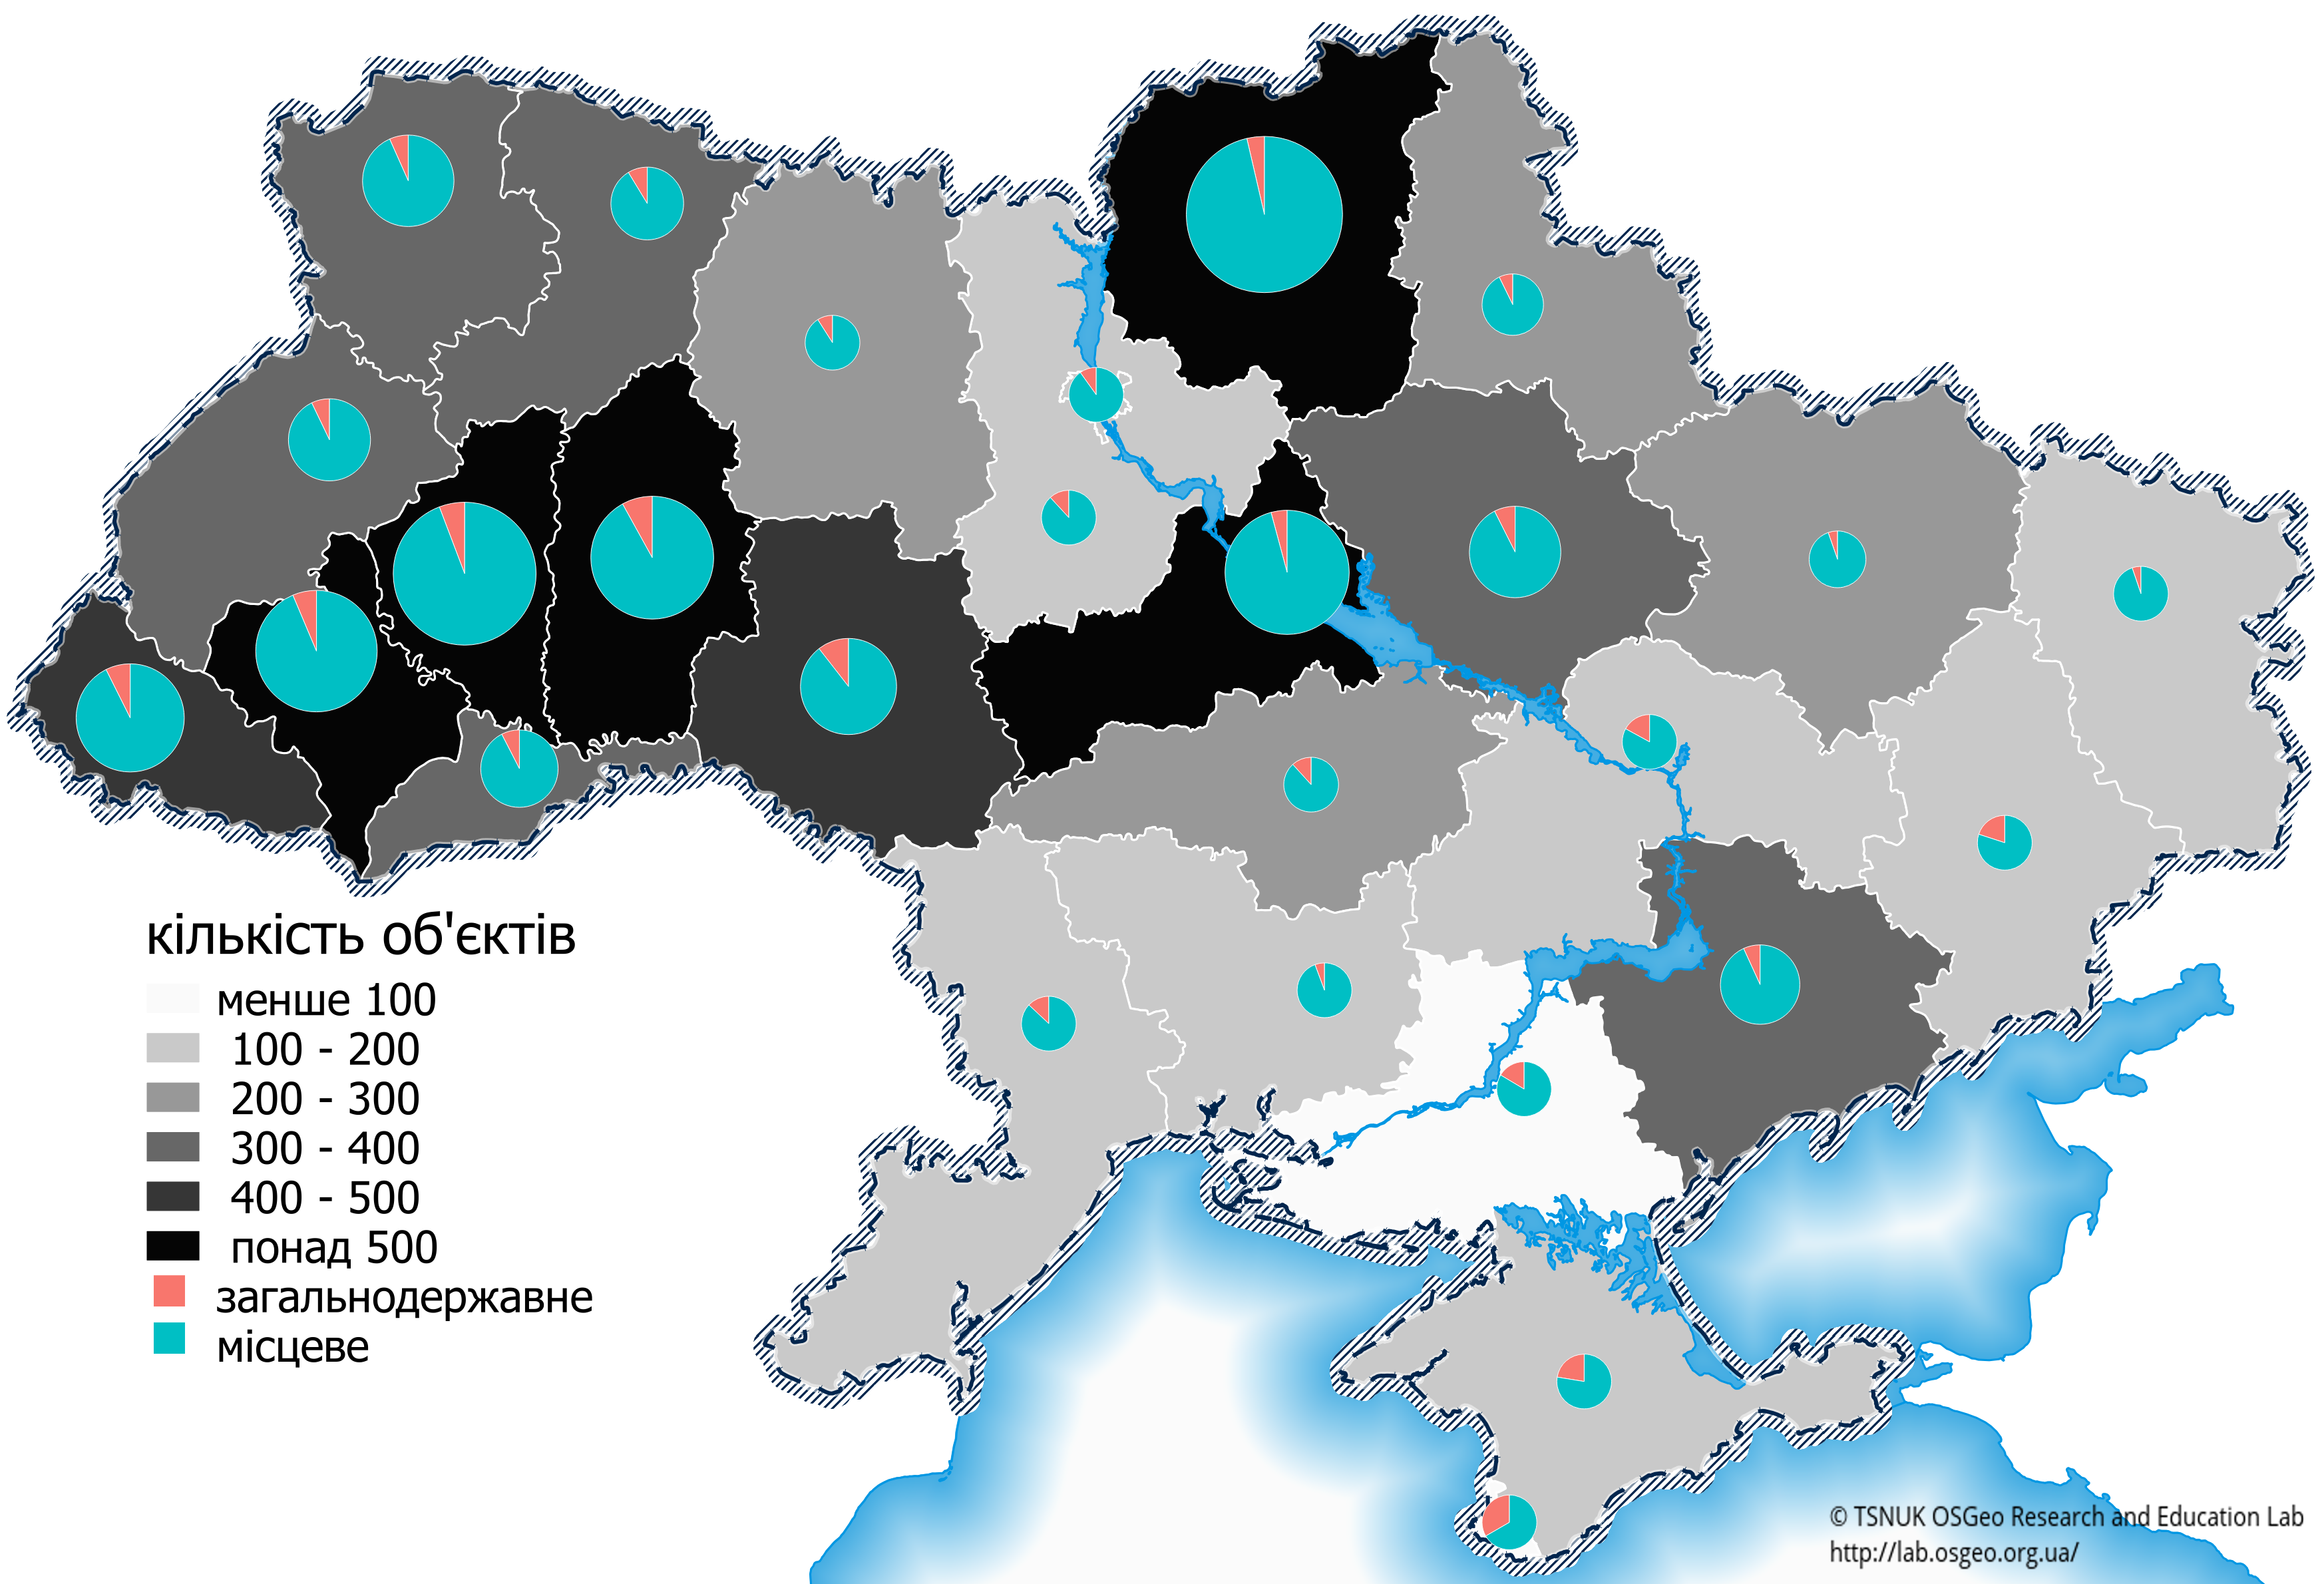
\includegraphics[width=\textwidth]{./figures/objects_count.png}%
		
		\column{.5\textwidth}
		
		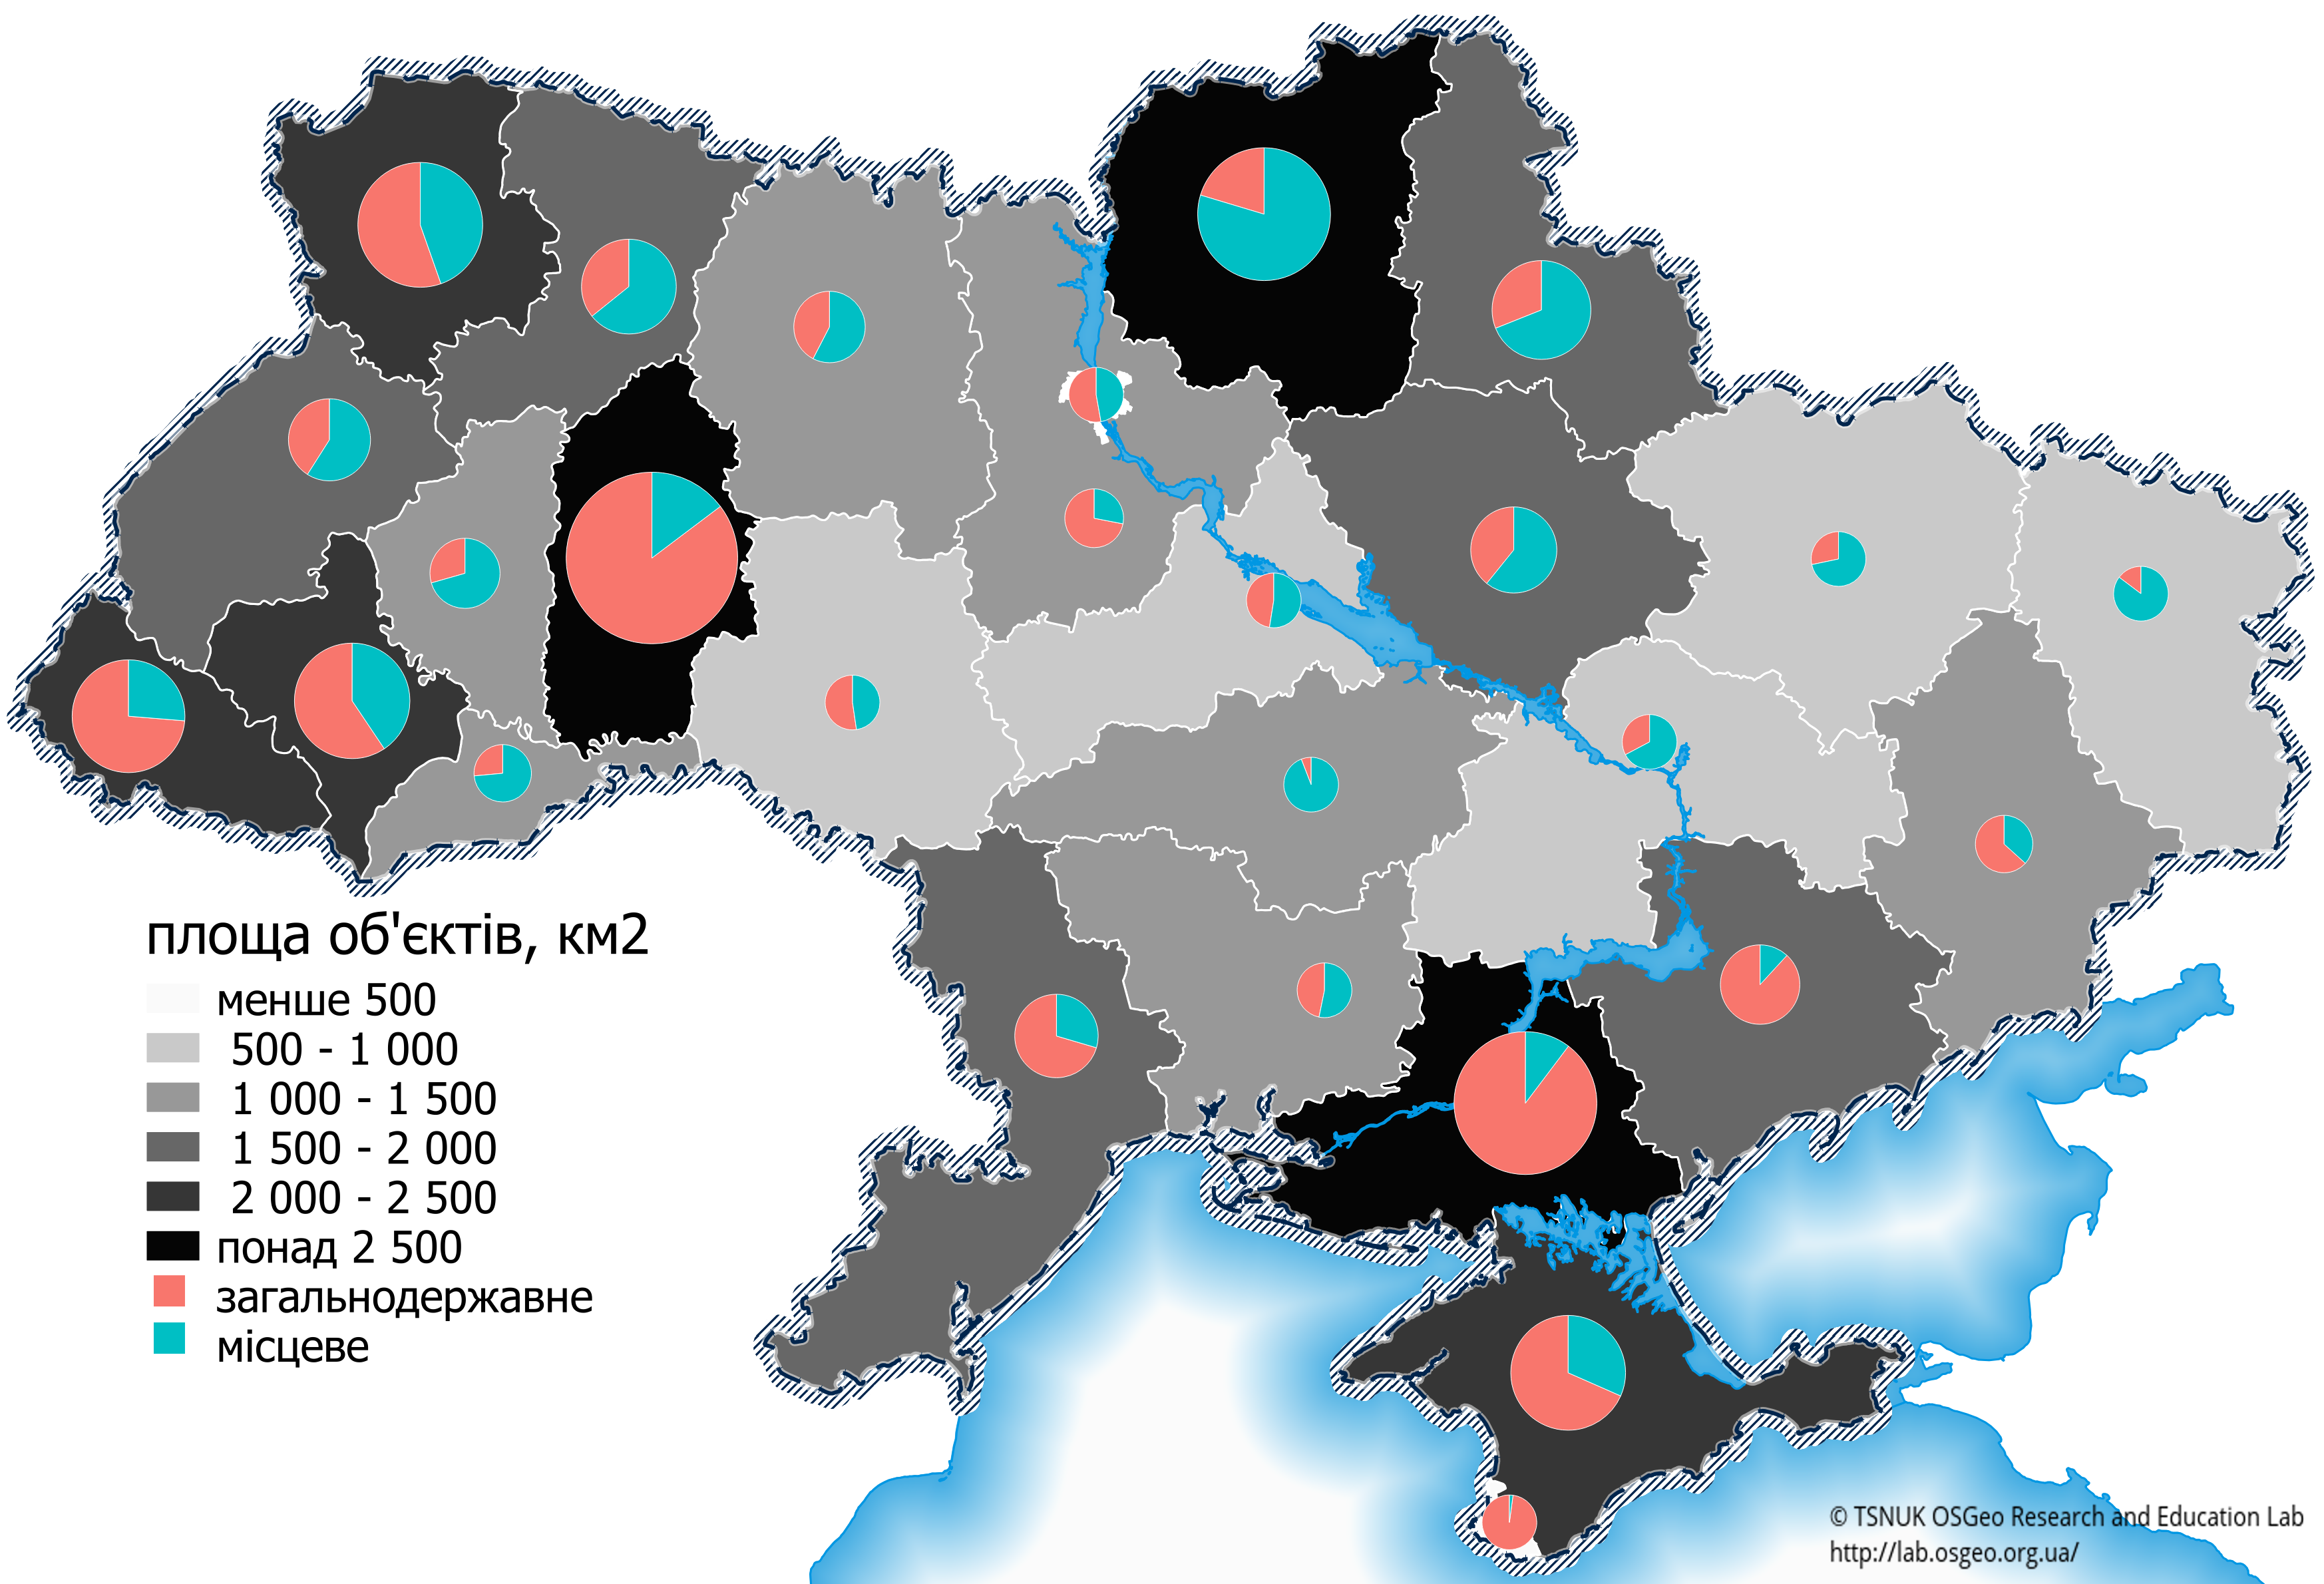
\includegraphics[width=\textwidth]{./figures/objects_area.png}
		
	\end{columns}
\begin{itemize}
	\item кількісно переважають об'єкти місцевого значення, а великі площі пов'язані з об'єктами загальнодержавного значення
	\item Чернігівська область -- переважання об'єктів місцевого значення як за кількістю, так і за площею
	\item Херсонська область -- невелика кількість об'єктів при значній площі
\end{itemize}
\end{frame}


\subsection{Як розподіляються об'єкти за категоріями?}
\begin{frame}{Структура природно-заповідного фонду}{Як розподіляються об'єкти за категоріями?}
	\begin{columns}[c]
		
		\column{.5\textwidth}
		
		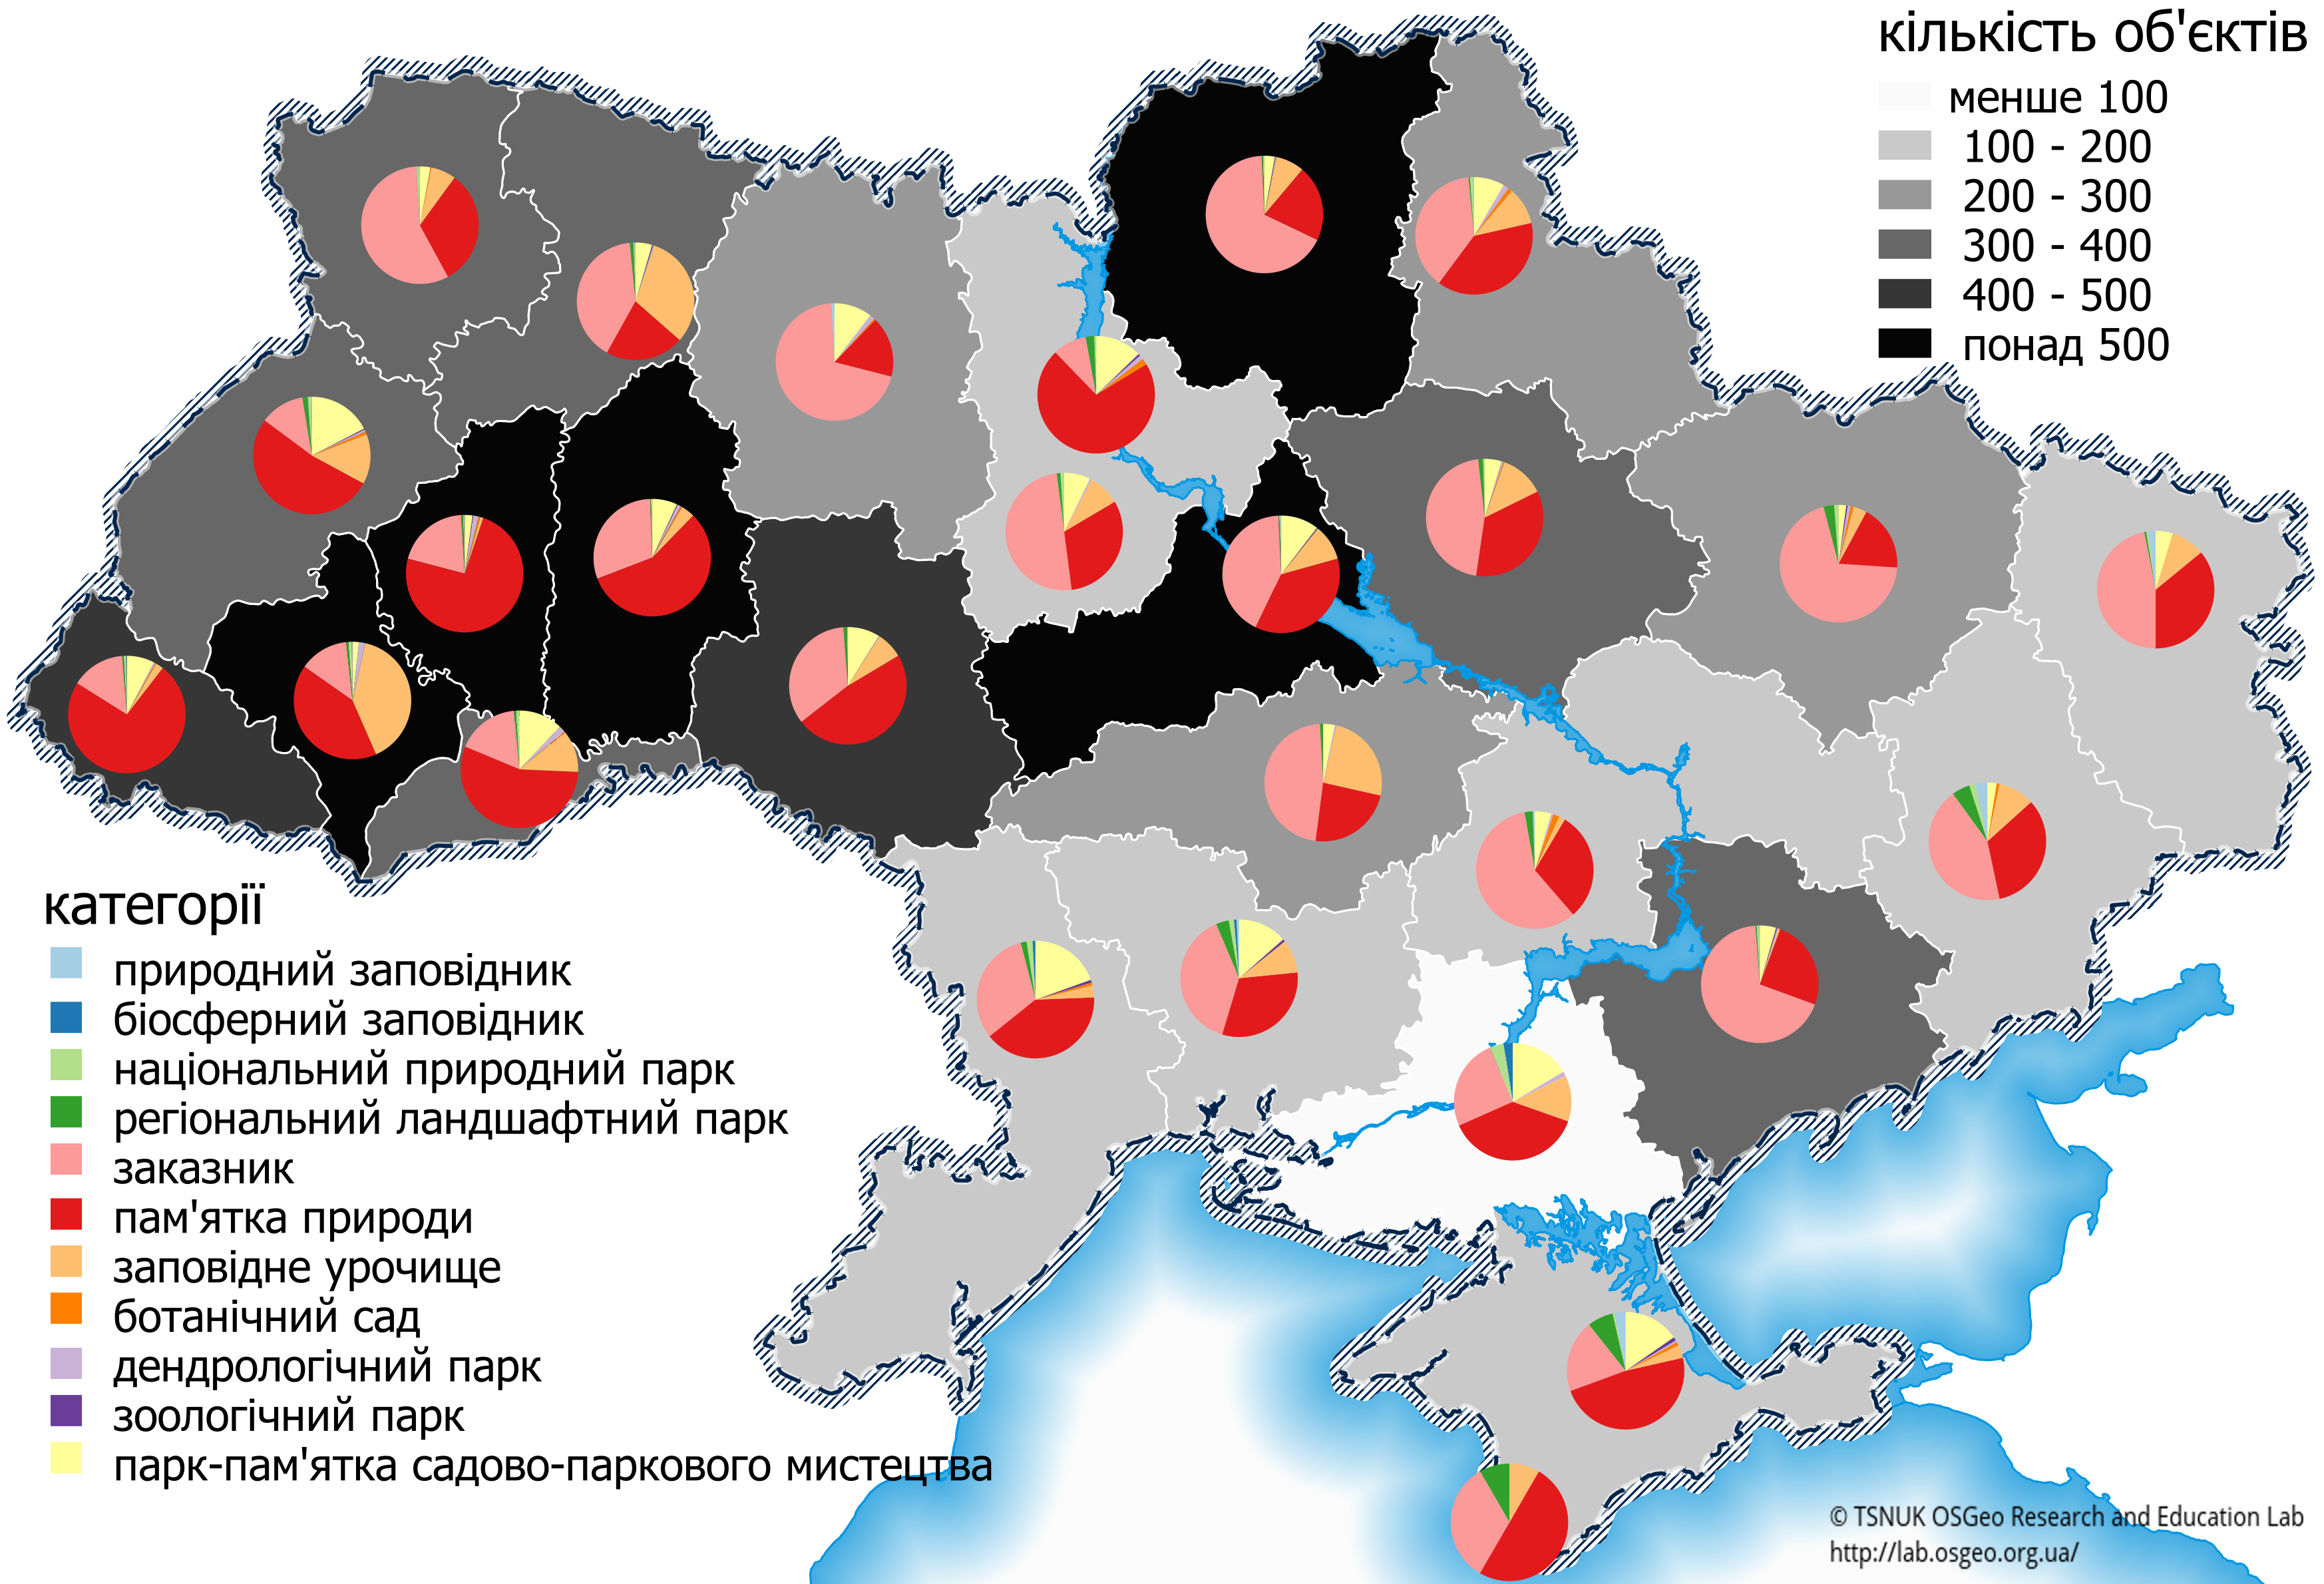
\includegraphics[width=\textwidth]{./figures/categories_count.png}%
		
		\column{.5\textwidth}
		
		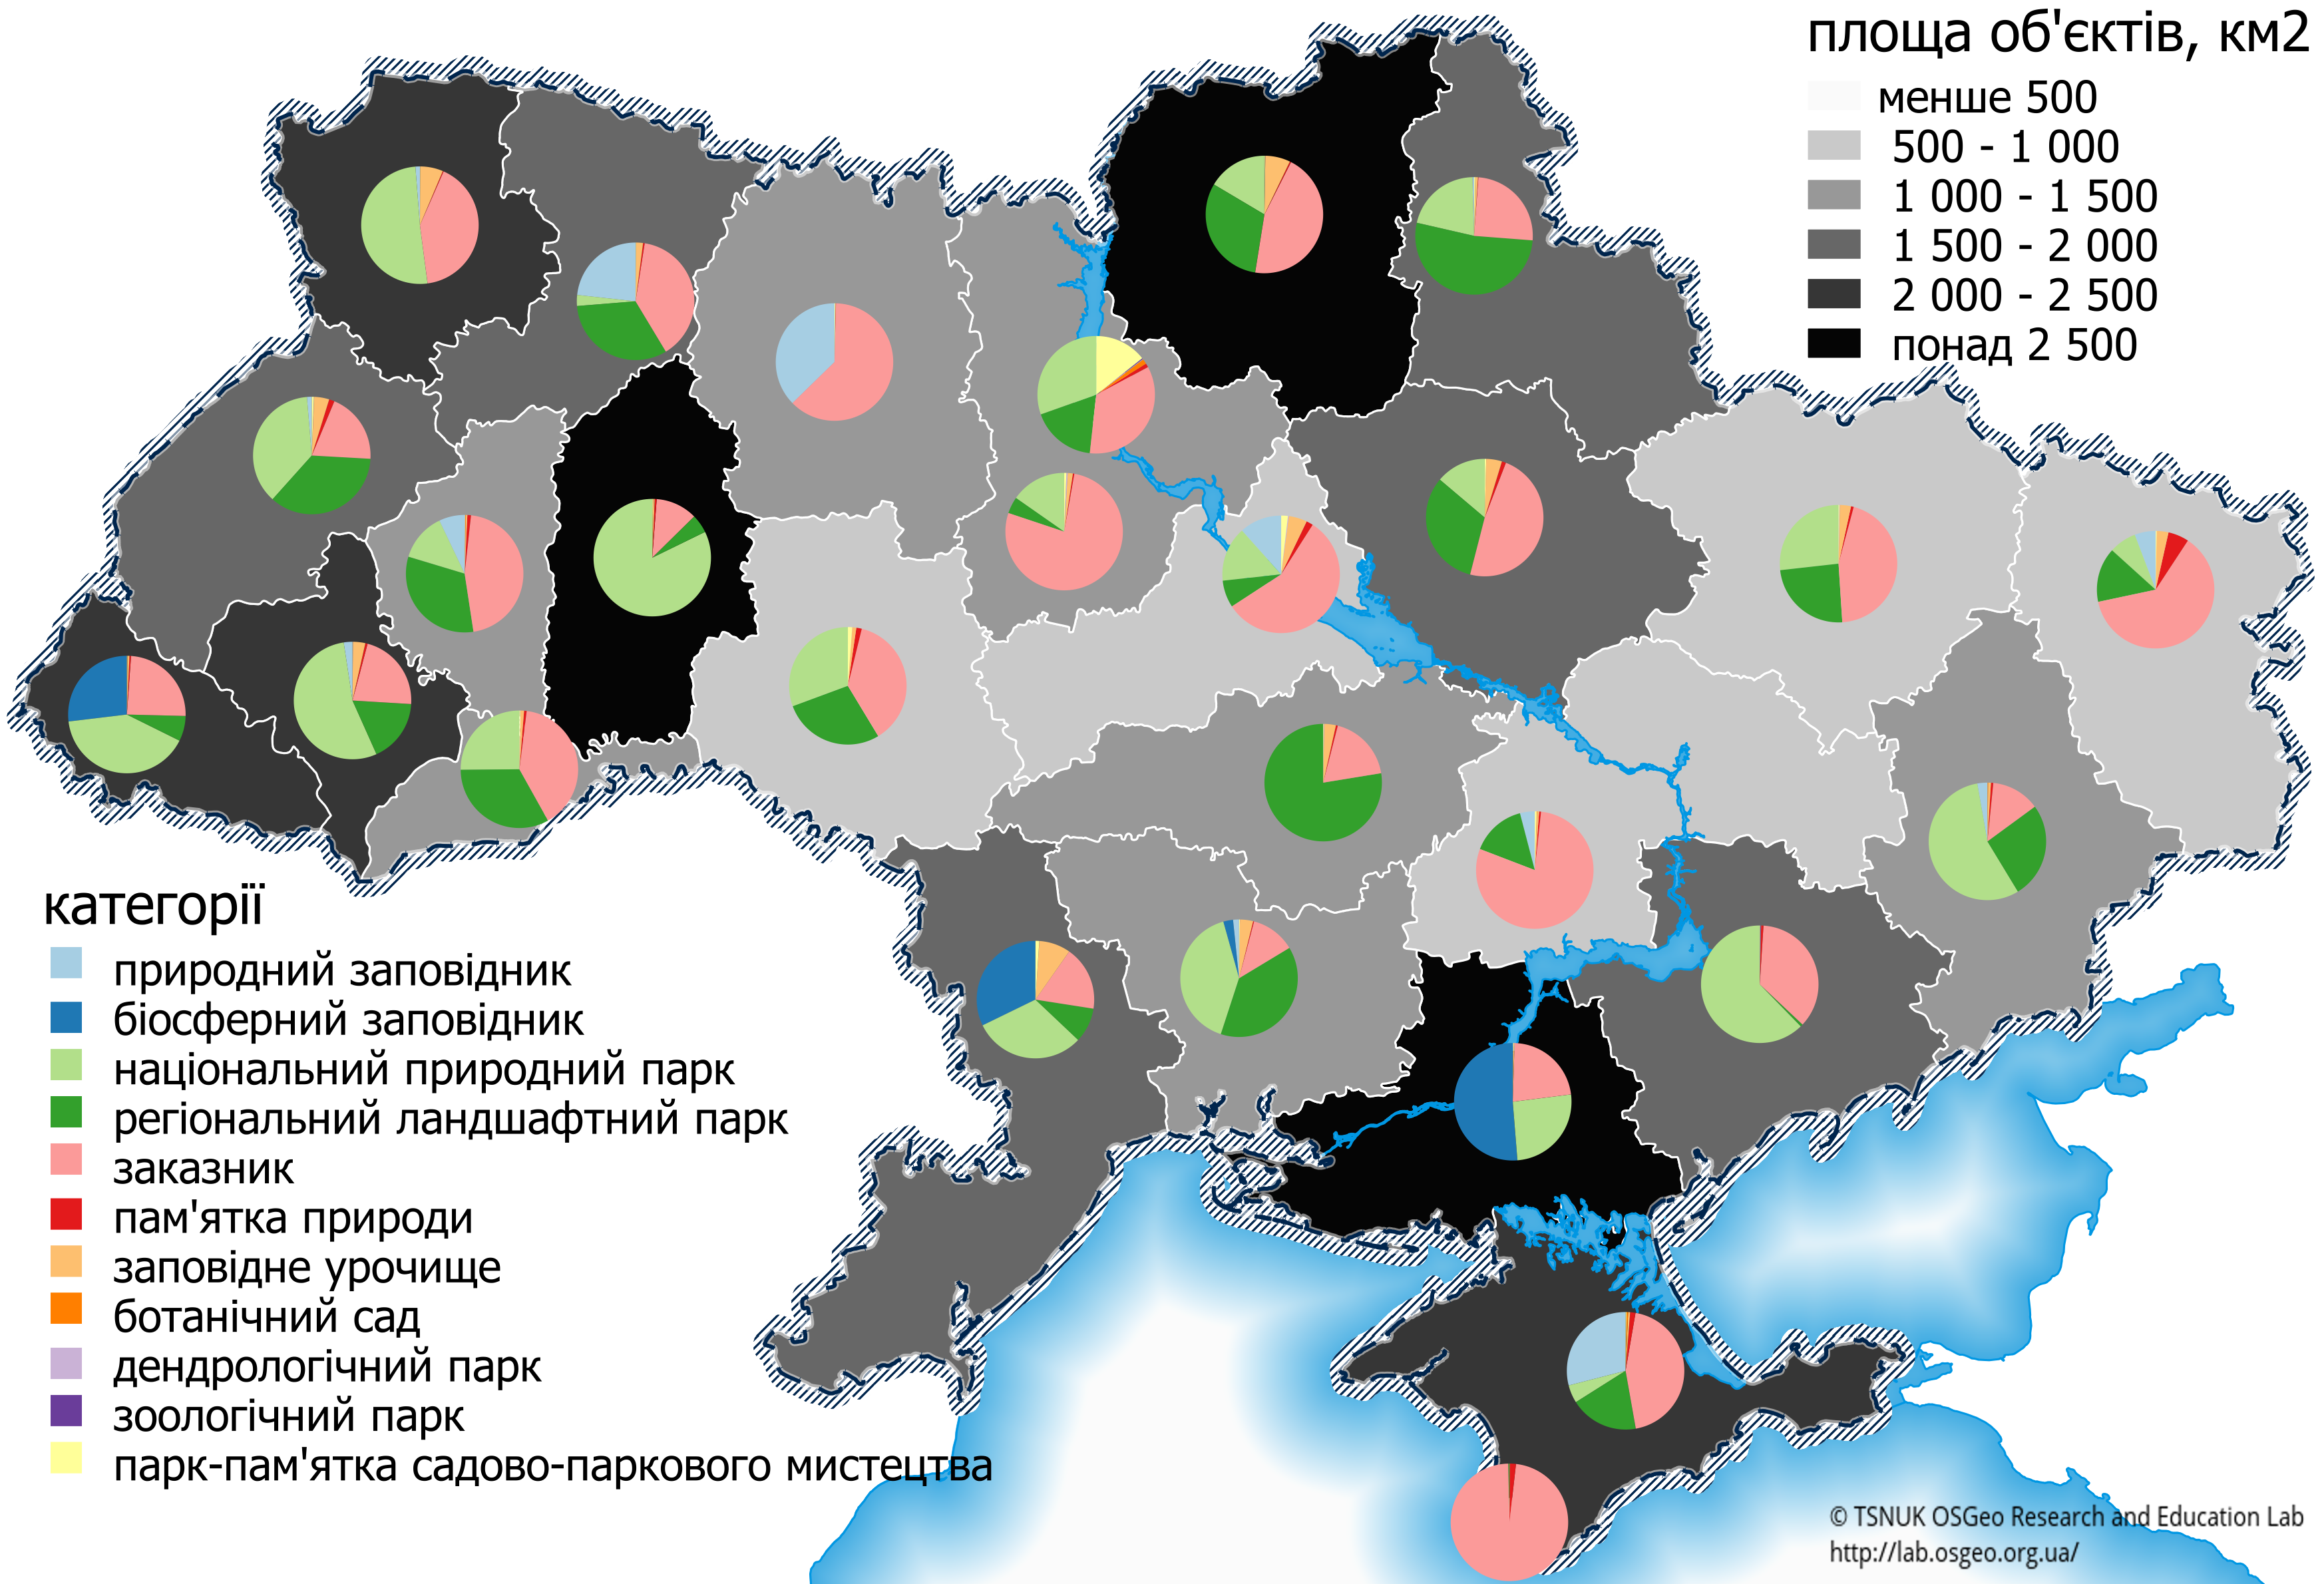
\includegraphics[width=\textwidth]{./figures/categories_area.png}
		
	\end{columns}
\begin{itemize}
	\item кількісно переважають пам'ятки природи та заказники
	\item за площею переважають заказники, національні природні парки та регіональні ландшафтні парки
\end{itemize}
\end{frame}


\subsection{Як розподіляються об'єкти загальнодержавного значення за категоріями?}
\begin{frame}{Структура природно-заповідного фонду}{Як розподіляються об'єкти загальнодержавного значення за категоріями?}
	\begin{columns}[c]
		
		\column{.5\textwidth}
		
		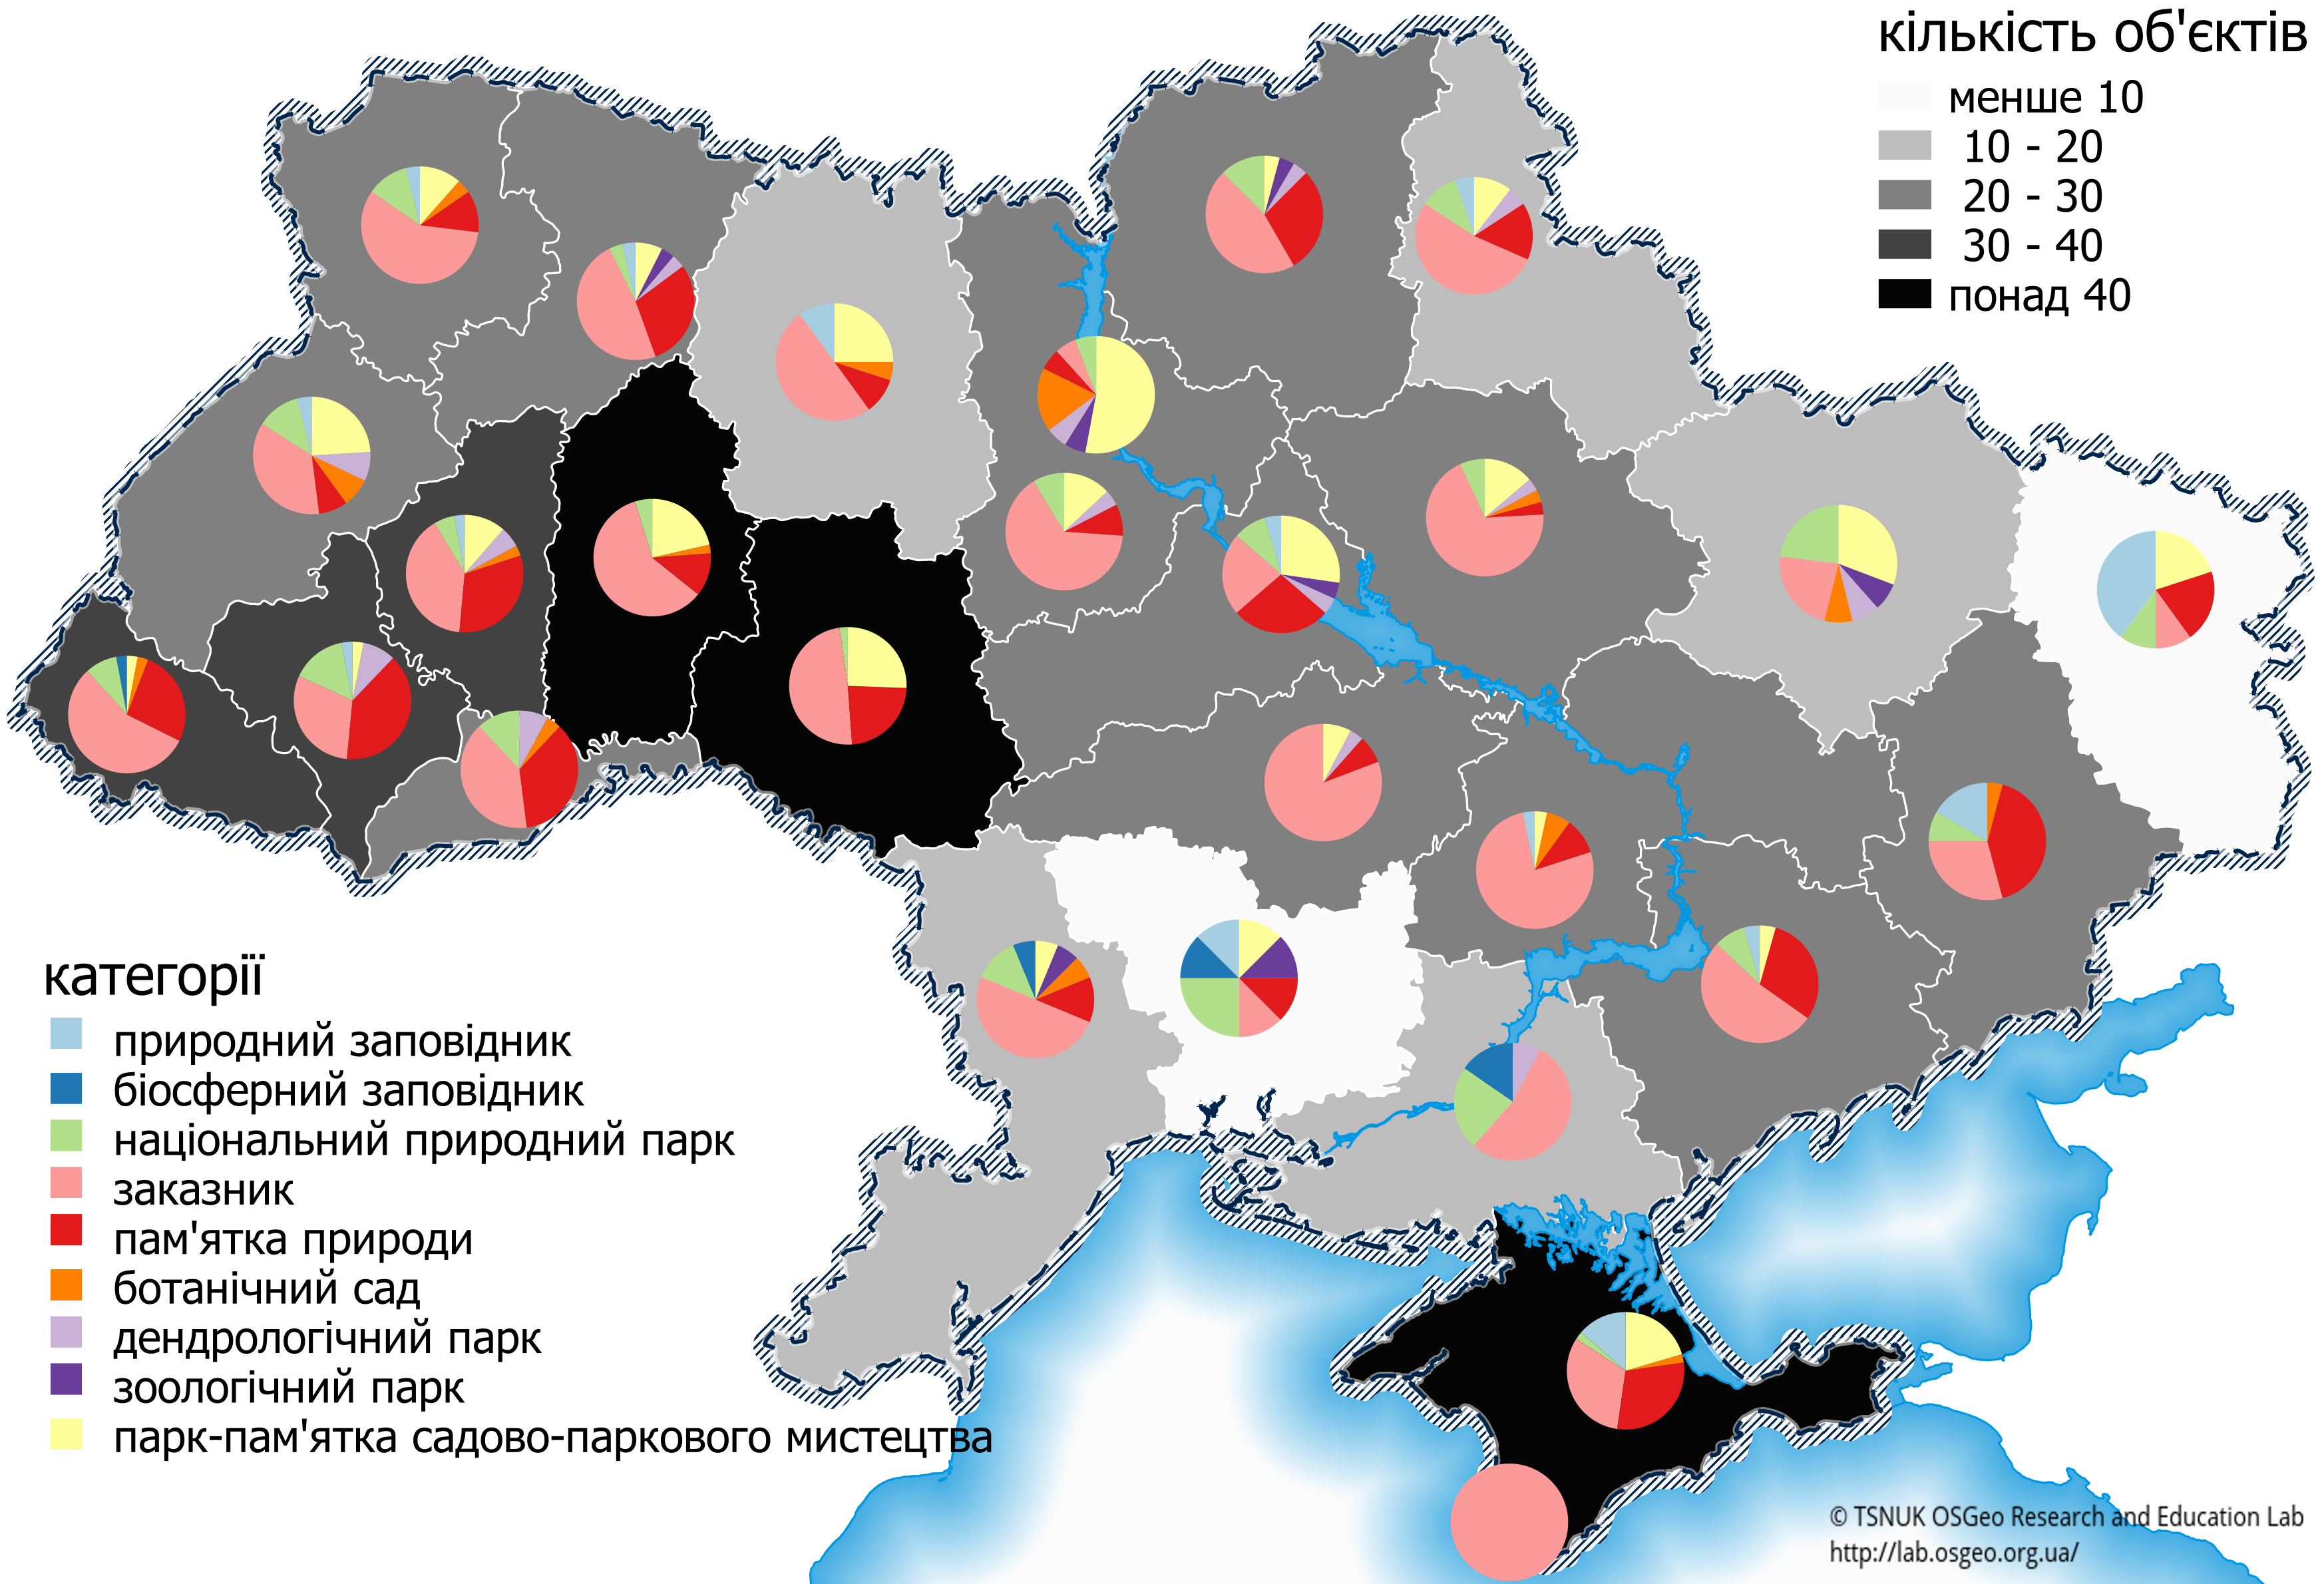
\includegraphics[width=\textwidth]{./figures/state_categories_count.png}%
		
		\column{.5\textwidth}
		
		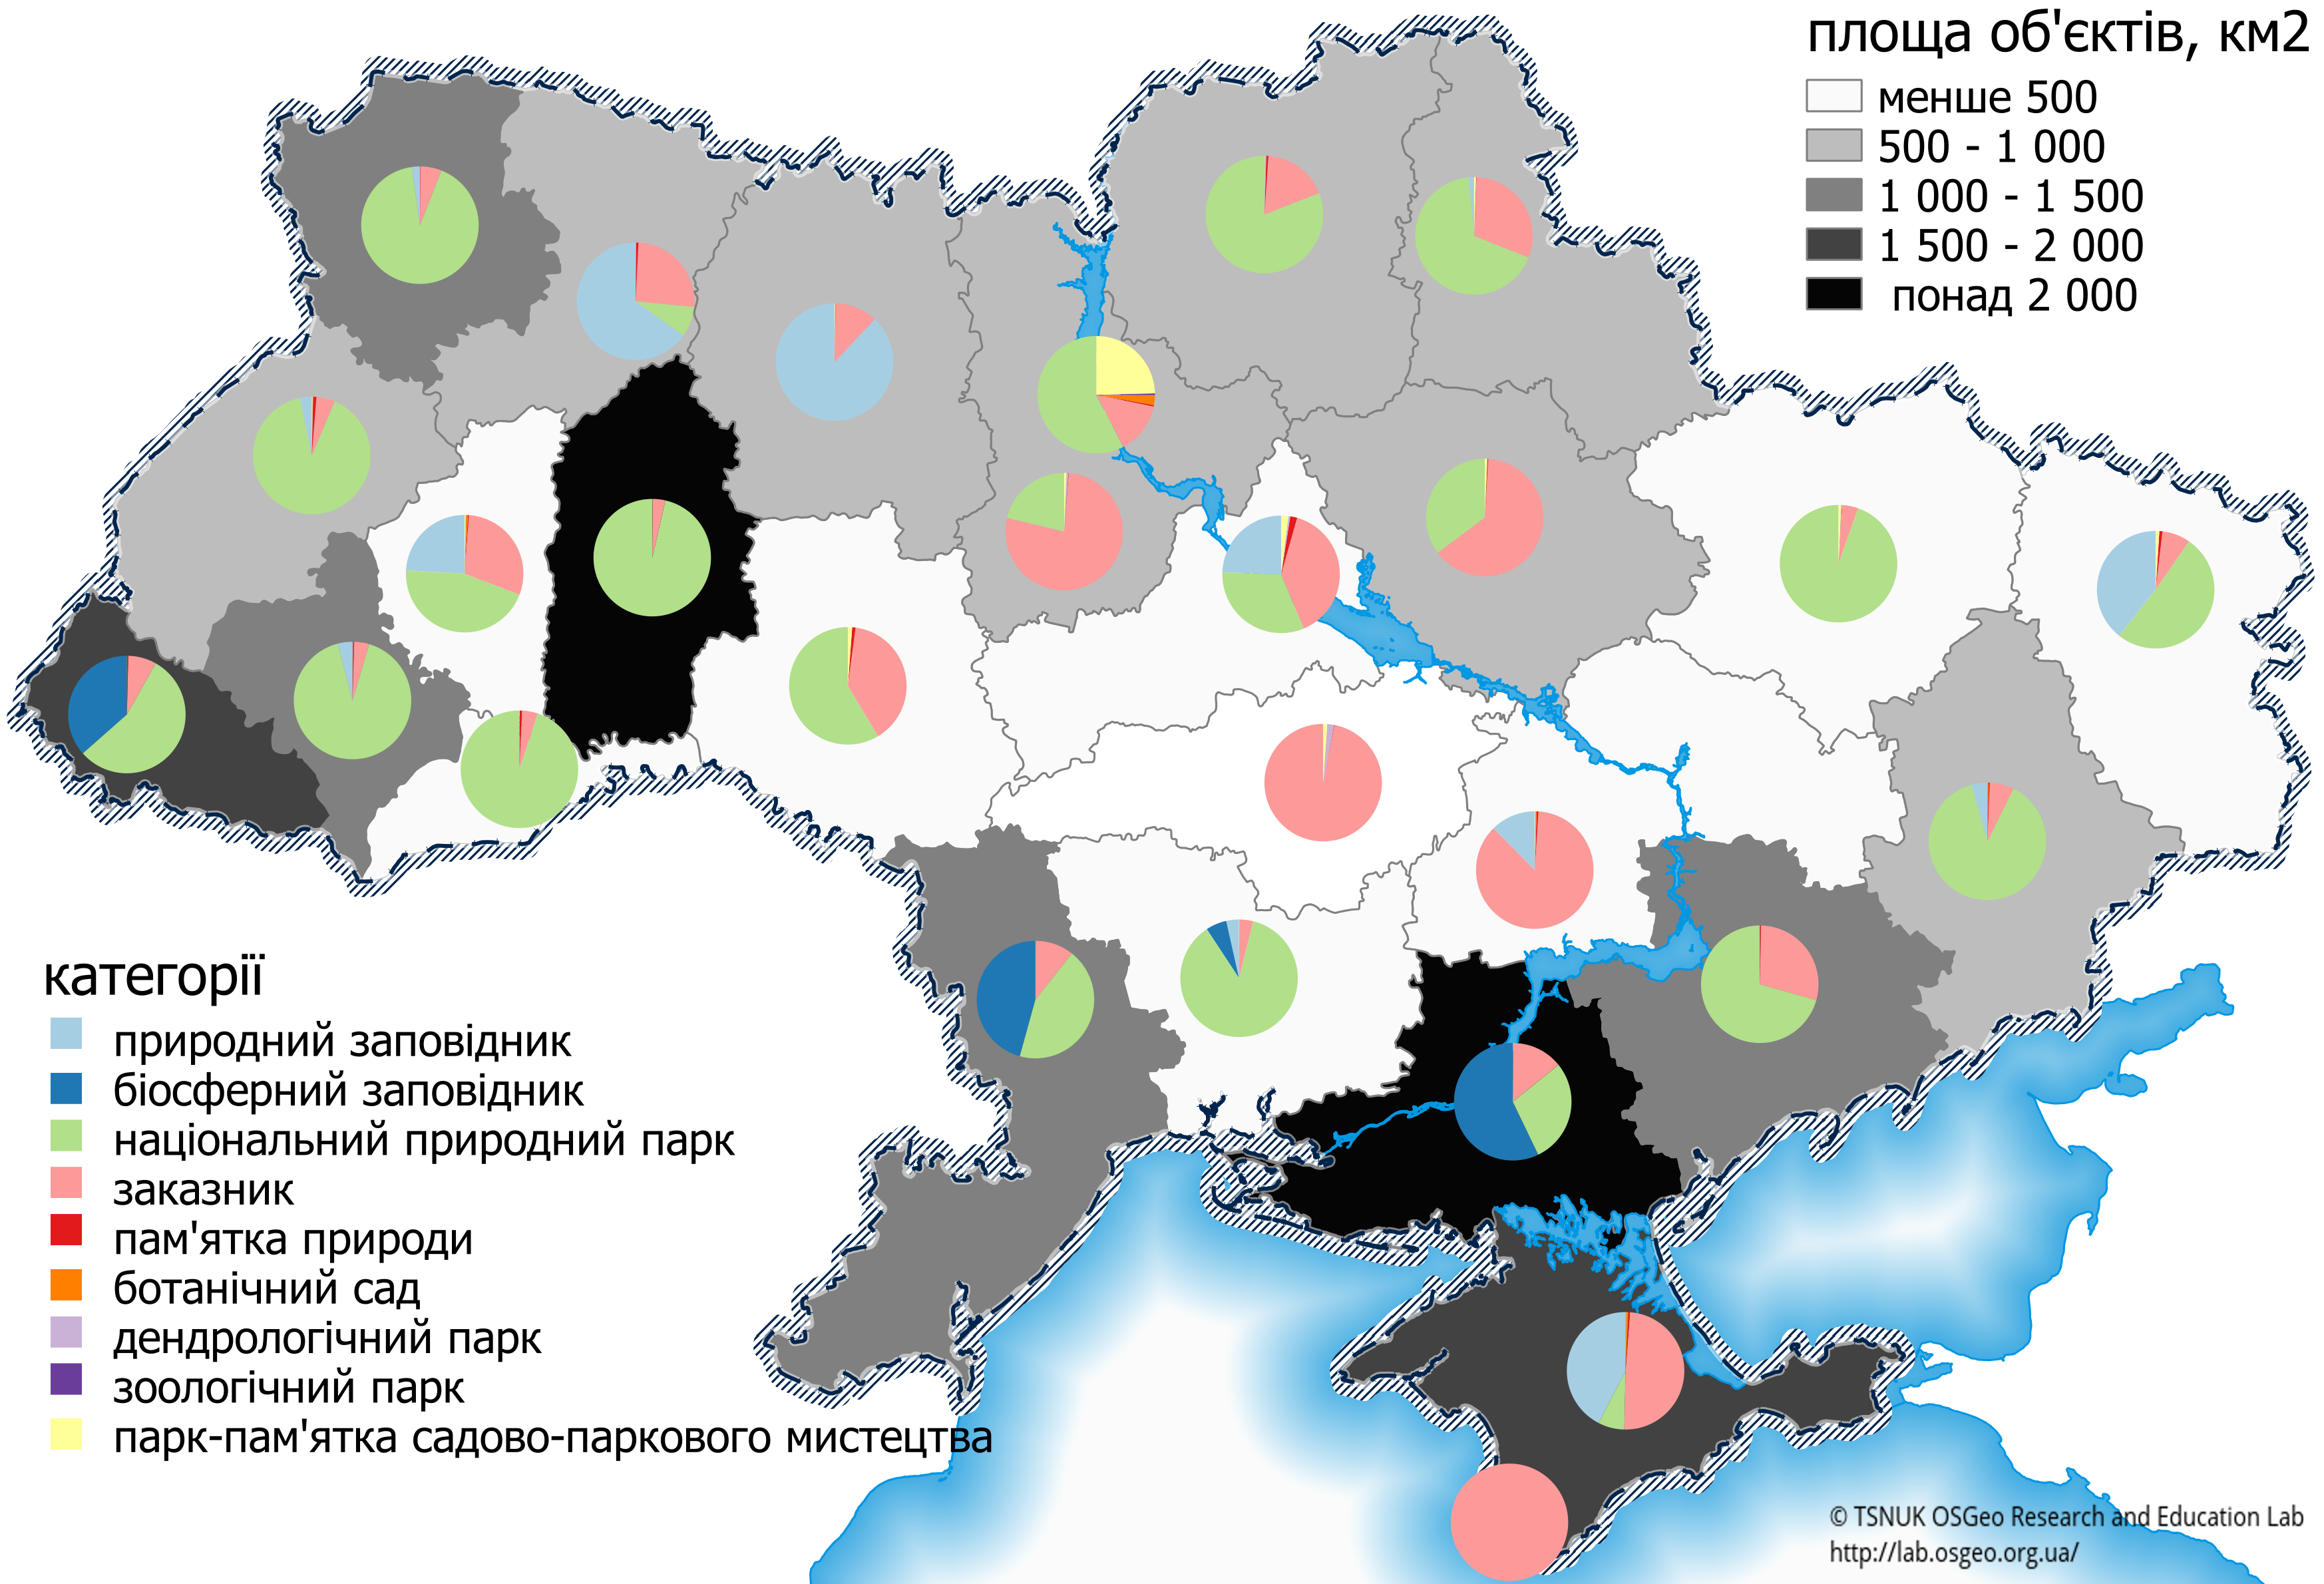
\includegraphics[width=\textwidth]{./figures/state_categories_area.png}
		
	\end{columns}
\begin{itemize}
	\item кількісно переважають заказники, пам'ятки природи, парки-пам'ятки садово-паркового мистецтва 
	\item за площею переважають національні природні парки, заказники та(або) заповідники
\end{itemize}
\end{frame}

\subsection{Як розподіляються об'єкти місцевого значення за категоріями?}
\begin{frame}{Структура природно-заповідного фонду}{Як розподіляються об'єкти місцевого значення за категоріями?}
	\begin{columns}[c]
		
		\column{.5\textwidth}
		
		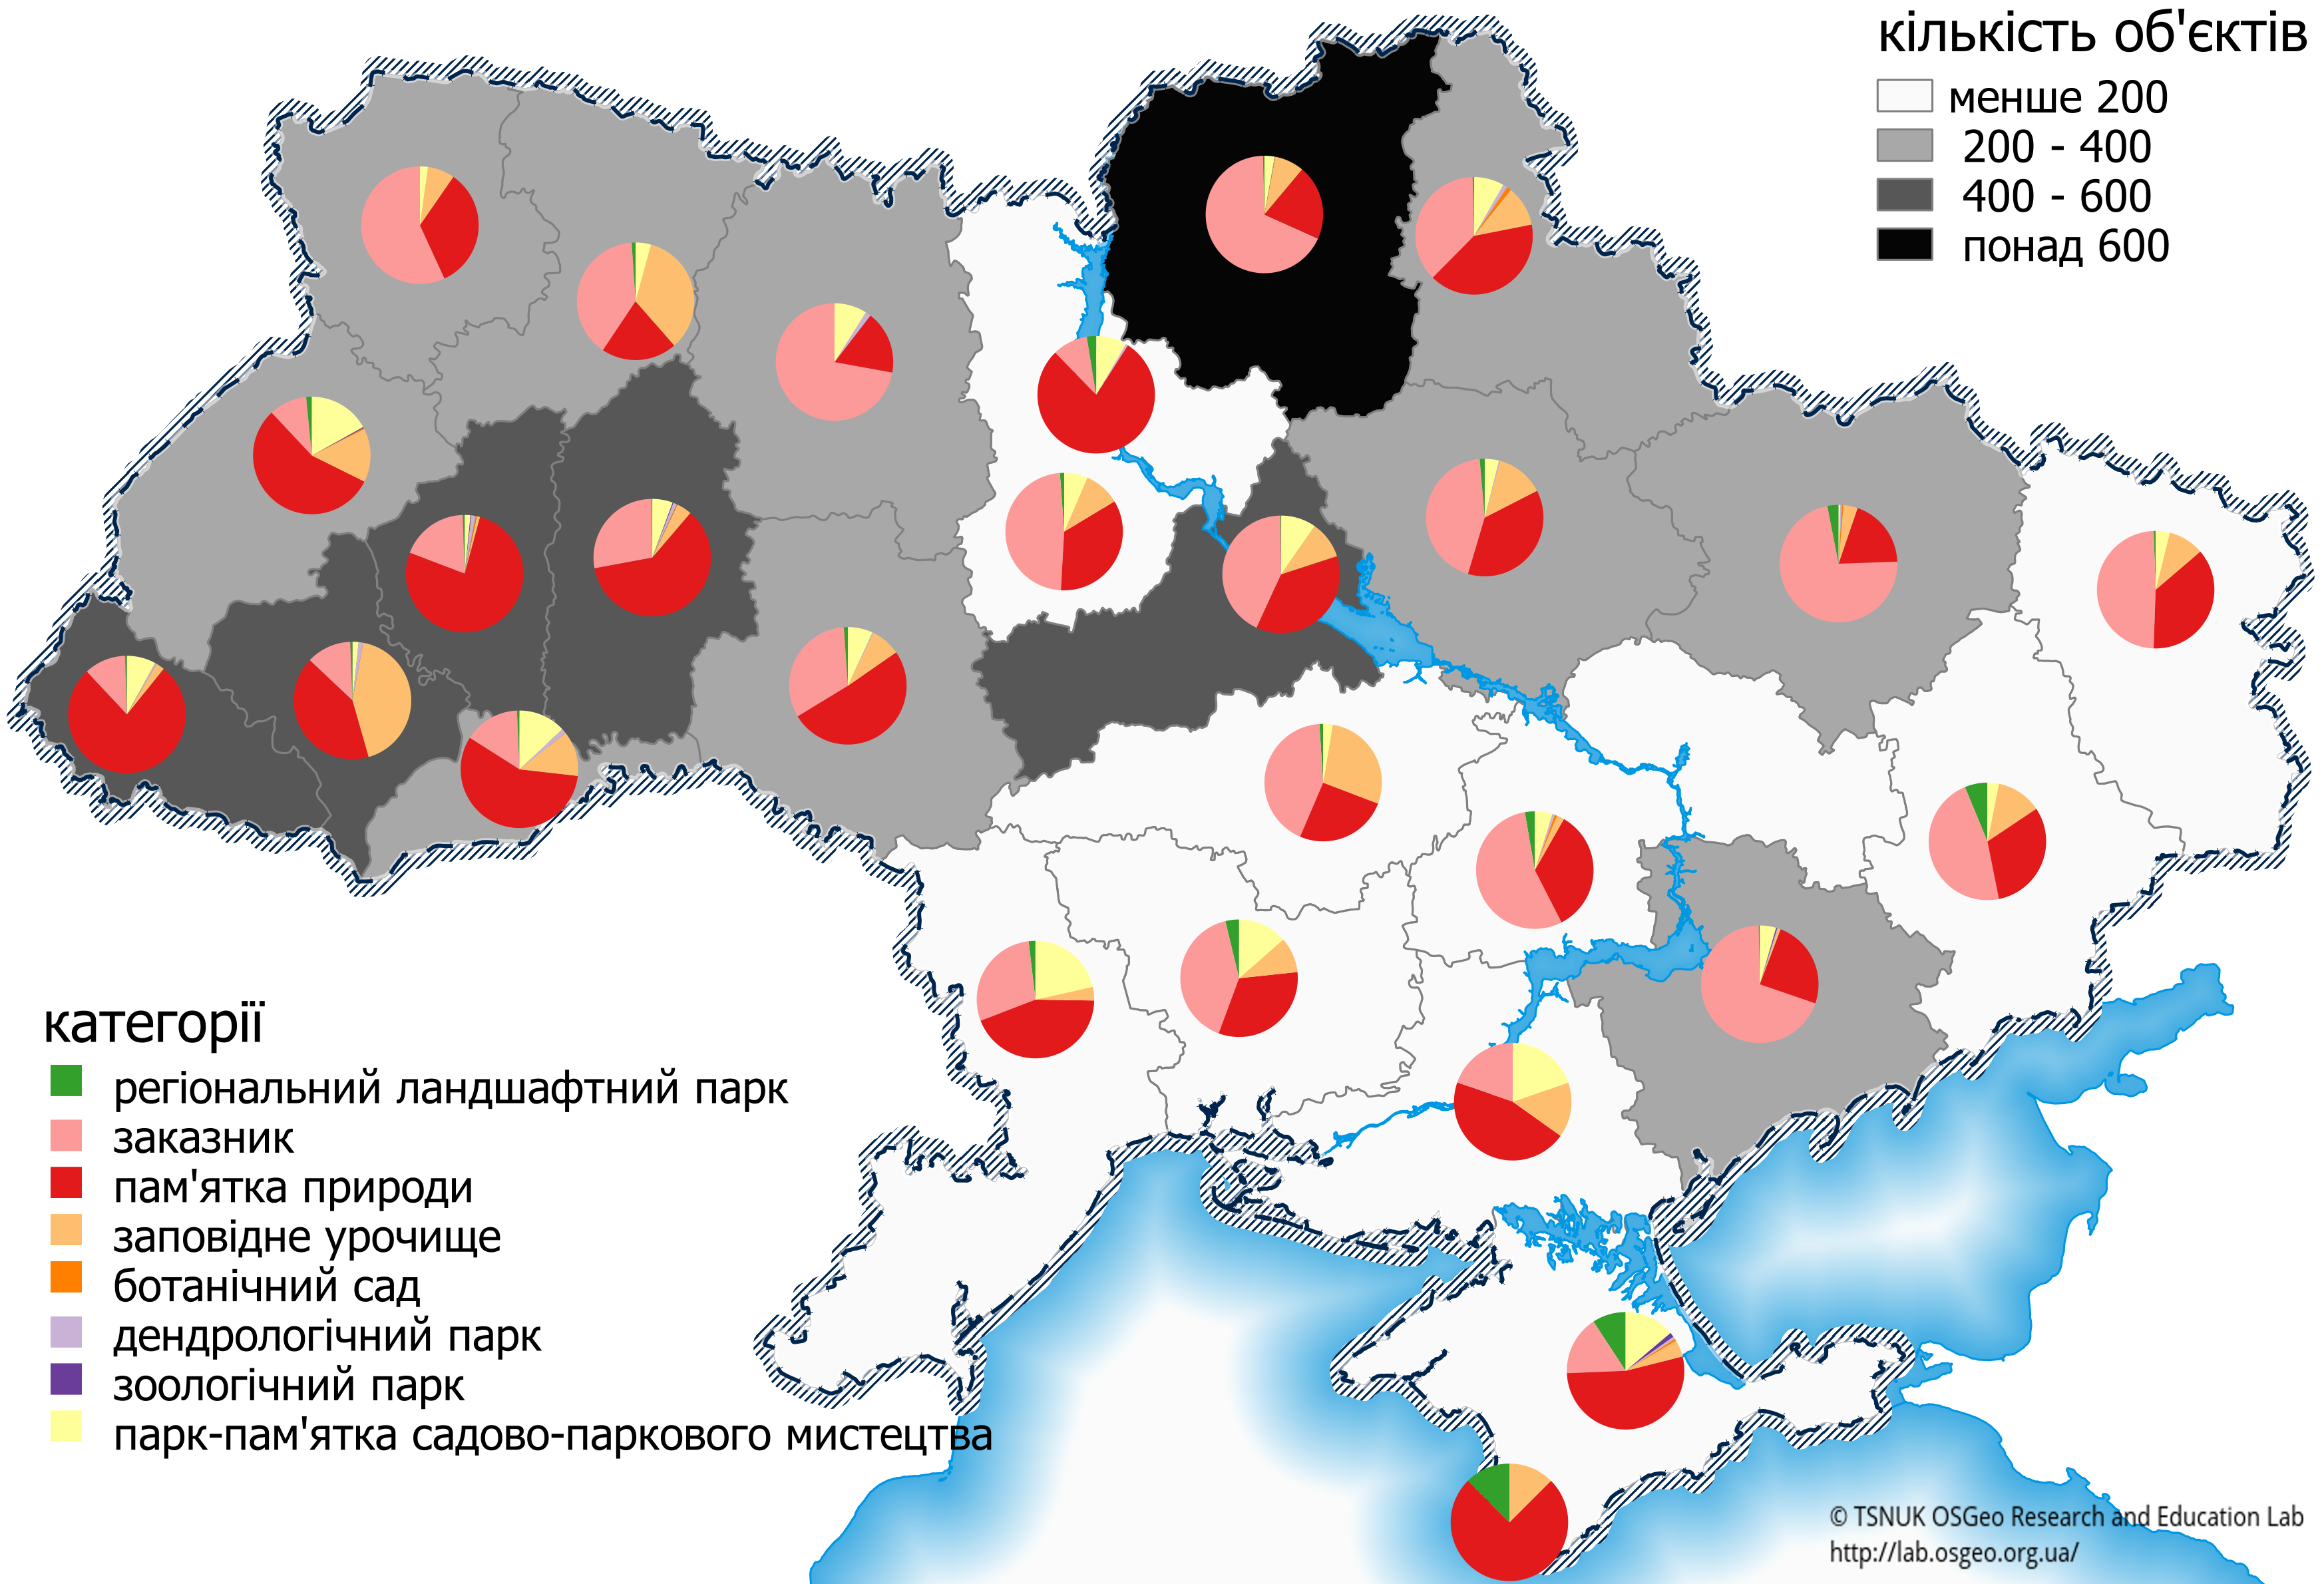
\includegraphics[width=\textwidth]{./figures/local_categories_count.png}%
		
		\column{.5\textwidth}
		
		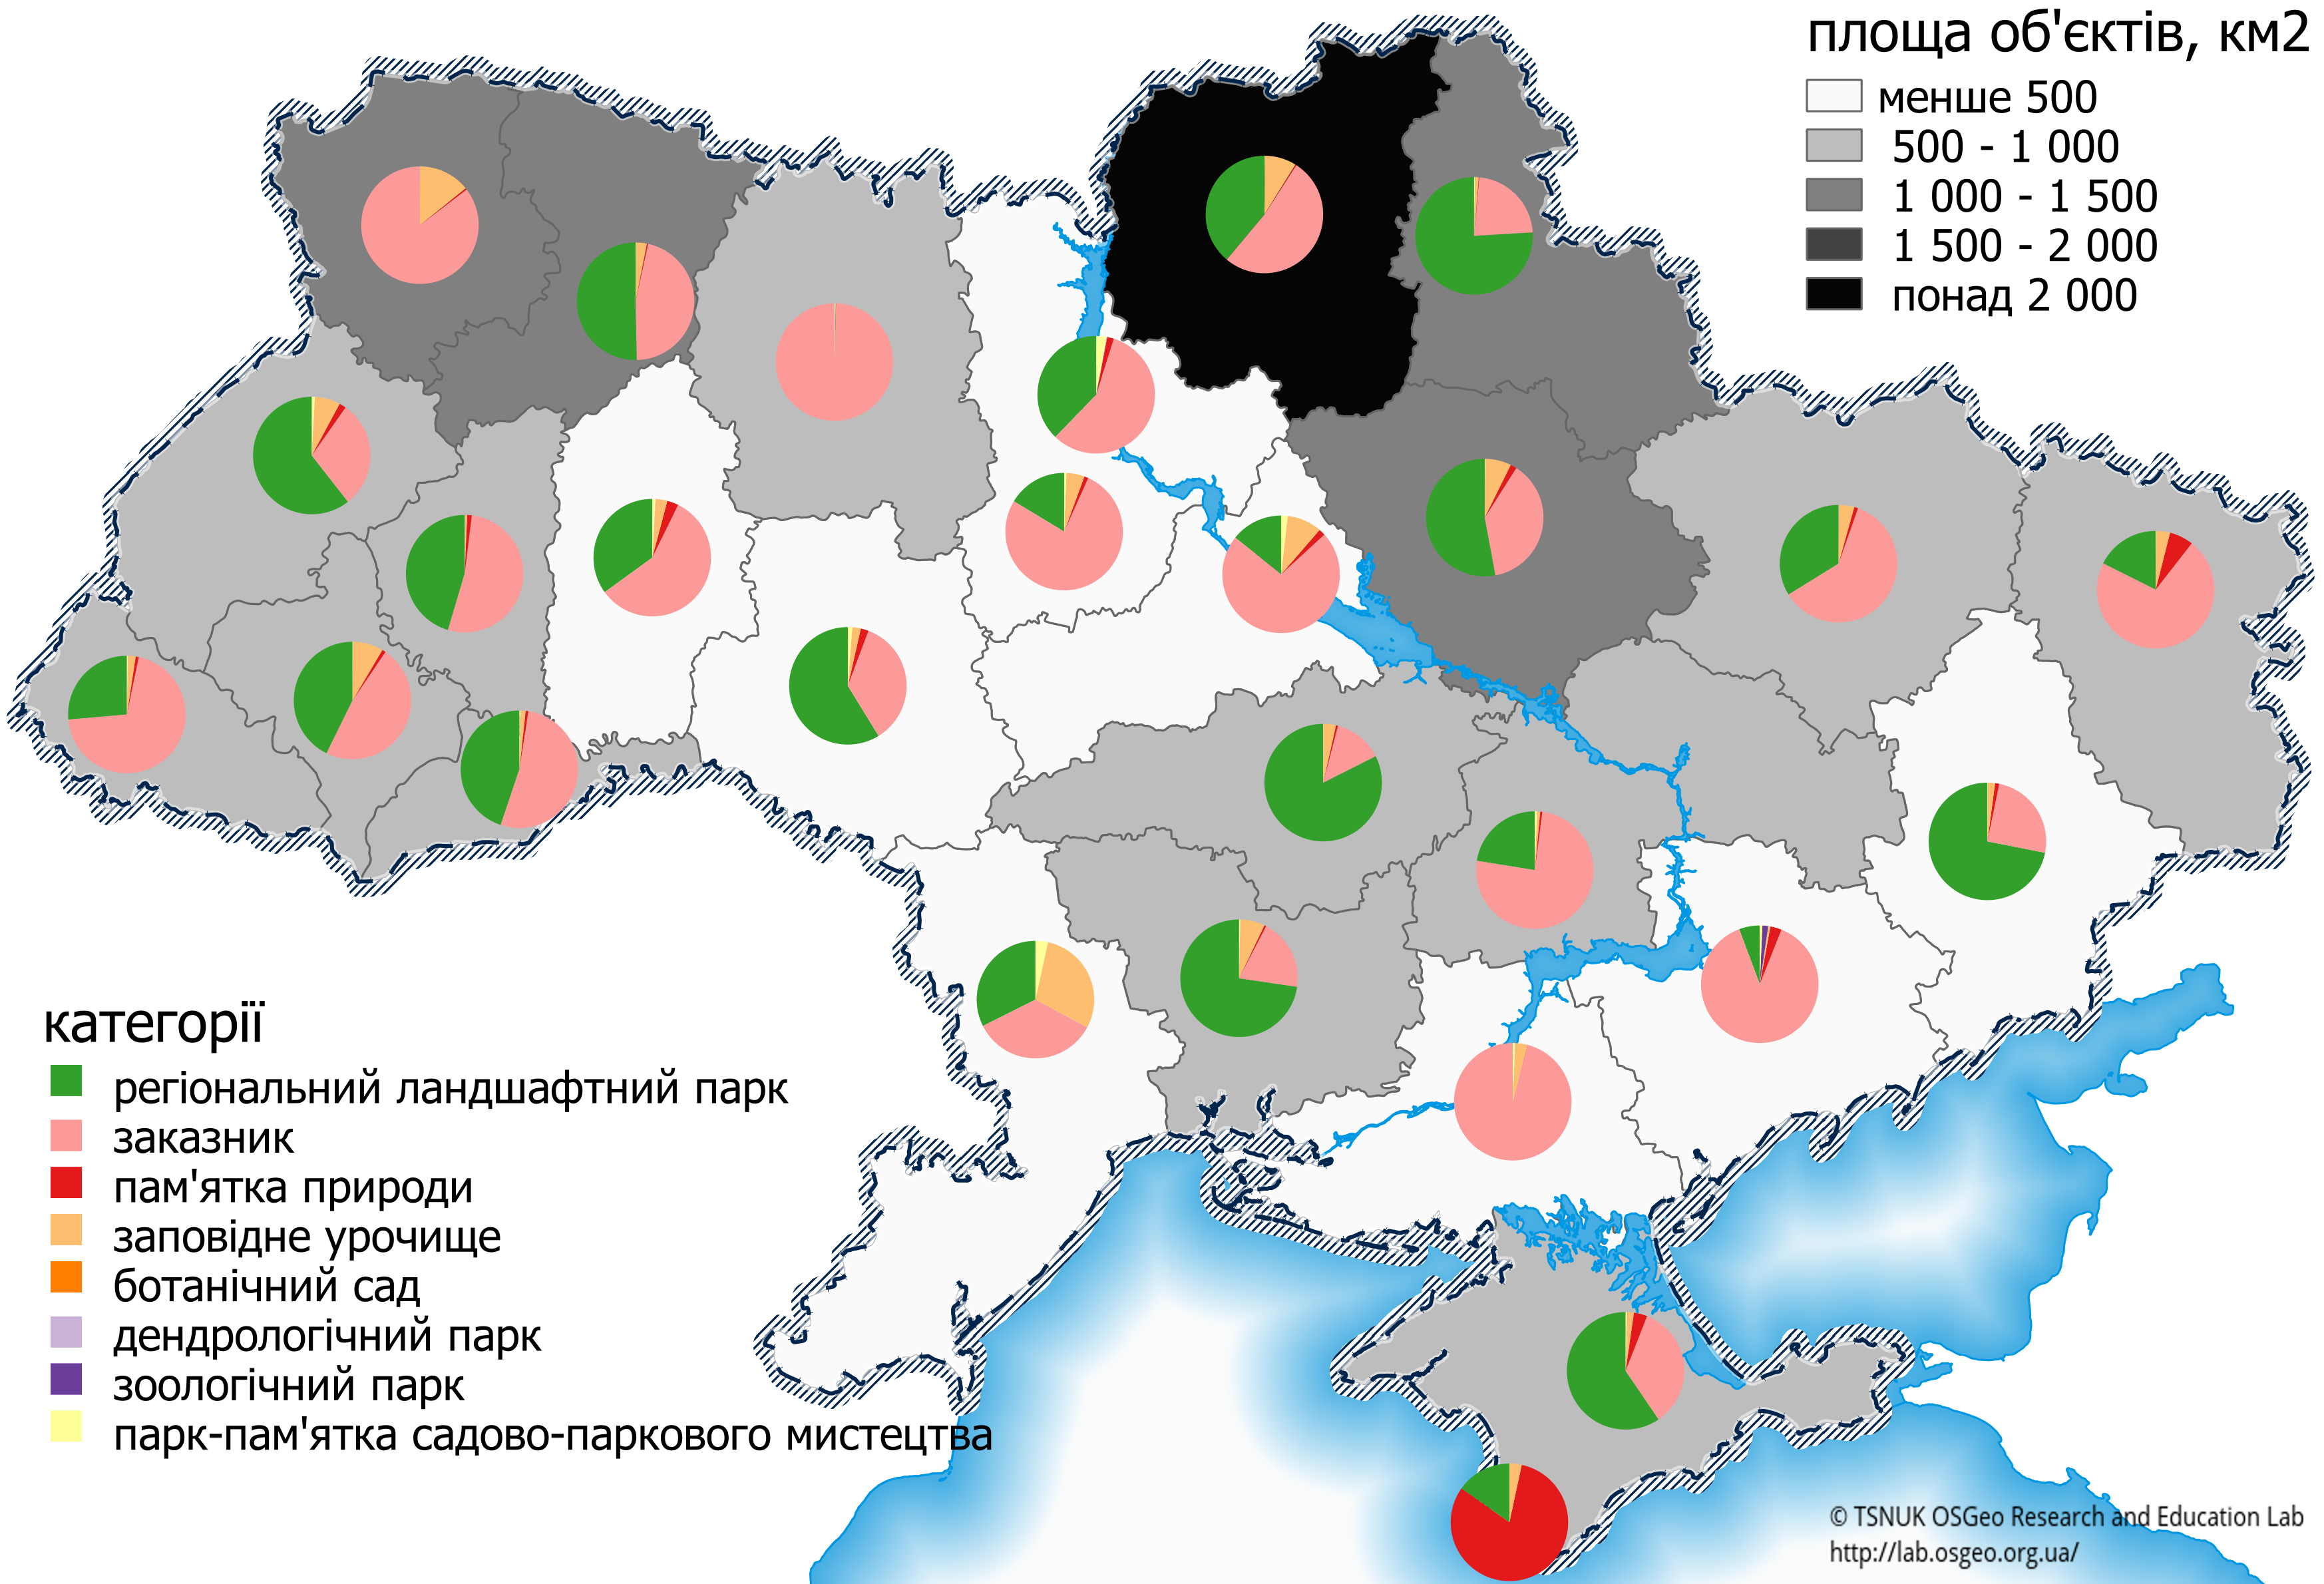
\includegraphics[width=\textwidth]{./figures/local_categories_area.png}
		
	\end{columns}
\begin{itemize}
	\item кількісно переважають пам'ятки природи, заказники
	\item за площею переважають  заказники, регіональні ландшафтні парки
\end{itemize}
\end{frame}


\section{Висновки}
\begin{frame}{Висновки}{}
  \begin{itemize}
    \item основна проблема при роботі з даними --- їх низька якість
    \item важливу роль в структурі природно-заповідного фонду відіграють заказники
    \item для адекватних оцінок заповідності необхідна інформація по вкладених територіях
  \end{itemize}
\end{frame}
%%%%%%%%%%%%%%%%


{%\aauwavesbg%
\begin{frame}[plain,noframenumbering]%
  \finalpage{Дякую за увагу!}
\end{frame}}
%%%%%%%%%%%%%%%%

\end{document}